\documentclass[11pt,a4paper]{article}
\usepackage[utf8]{inputenc}
\usepackage[italian]{babel}
\usepackage{amsmath}
\usepackage{amsfonts}
\usepackage{amssymb}
\usepackage{array}
\usepackage{graphicx}
\usepackage{multirow}
\usepackage{color,colortbl}
\usepackage[hidelinks]{hyperref}
\usepackage{fancyhdr}
\usepackage{tabularx}
\usepackage[left=2cm,right=2cm,top=2cm,bottom=2cm]{geometry}


\pagestyle{fancy}
\lhead{
\includegraphics[scale=0.08]{images/logo.png}}

\usepackage{appendix}
\usepackage{longtable}

\definecolor{LightBlue}{rgb}{0,0,0.5}
\definecolor{Gray}{gray}{0.8}
\definecolor{LightGray}{gray}{0.9}

\begin{document}
	\begin{titlepage}
  \centering
	\scshape
	
	\vspace*{2cm}
	
\includegraphics[scale=0.7]{images/logo.png}
	\rule{\linewidth}{0.2mm}\\[0.37cm]
	{\Huge Piano di progetto}\\
	\rule{\linewidth}{0.2mm}\\[1cm]
	{\LARGE\bfseries Progetto Colletta - Gruppo OttoBit}\\[1cm]
	
	
	
	\begin{tabular}{>{\columncolor{Gray}}r | >{\normalfont}l}
		\rowcolor{LightBlue}		
		\multicolumn{2}{c}{\color{white}{Informazioni sul documento}}\\
		Versione & 1.0.0 \\
		Redazione & Benedetto Cosentino\\
							& Enrico Marcato\\
 		Verifica & Giovanni Peron\\
 		Responsabile & Benedetto Cosentino\\
 		Uso & Esterno\\
 																 		& Prof. Tullio Vardanega\\
 																		& Prof. Riccardo Cardin\\
 		\multirow[t]{-3}{*}{Destinatari}	& MIVOQ s.r.l\\
 		\hline
	\end{tabular}
\end{titlepage}

	\tableofcontents
	\newpage
	\section*{\centering Registro delle modifiche}
	\begin{tabularx}{\textwidth}{ c | c | c | c | X }
		\rowcolor{LightBlue}
		\color{white}\bfseries Versione & \color{white}\bfseries Data & \color{white}\bfseries Autore & \color{white}\bfseries Ruolo & \multicolumn{1}{c}{\color{white}\bfseries Descrizione}\\[0.25cm]
		0.0.3 & 2018/12/15 & Benedetto Cosentino & Responsabile & Aggiunta della pianificazione dell'analisi dei requisiti\\
		0.0.2 & 2018/12/14 & Benedetto Cosentino & Responsabile & Aggiunta del modello di sviluppo e migliorie alle sezioni precedenti\\
		0.0.1 & 2018/12/12 & Benedetto Cosentino & Responsabile & Creazione dello scheletro e aggiunta dell'introduzione e dell'analisi dei rischi\\
	\end{tabularx}

	\newpage	
	\section{Introduzione}
		\subsection{Scopo del documento}
	Il documento ha lo scopo di definire la pianificazione del progetto ``Colletta: piattaforma raccolta dati di analisi di testo" proposto da MIVOQ S.r.l. per il gruppo OttoBit. Il documento viene aggiornato durante le attività di incremento che lo riguardano ogniqualvolta è necessario. Al suo interno presenta:
	\begin{itemize}
		\item un'analisi dei rischi in cui è possibile incorrere;
		\item una breve analisi sul modello di sviluppo scelto;
		\item la pianificazione dei tempi e delle attività;
		\item l'assegnazione delle attività pianificate ai membri del team;
		\item una stima preventiva delle risorse;
		\item la rendicontazione delle risorse impiegate.
	\end{itemize}

\subsection{Scopo del prodotto}
	Il prodotto richiesto dalla proponente è una piattaforma che permetta la raccolta di dati in modo implicito tramite la risoluzione di esercizi. Tali dati devono essere utilizzati per addestrare un software di apprendimento automatico$^*$ già esistente che, a sua volta, deve essere in grado di fornire una soluzione agli esercizi proposti. L'obiettivo del prodotto potrà essere raggiunto tramite l'impiego di un database$^*$ che garantisca la permanenza dei dati, il software di apprendimento automatico e un'interfaccia (web o di un'applicazione mobile) che permetta l'interazione con gli utenti.

\subsection{Glossario}
	All'interno del documento è possibile trovare termini ambigui: in tal caso, tali termini possono essere trovati nel Glossario insieme alla relativa spiegazione. I termini del glossario vengono indicati con un * in apice.
	
\subsection{Riferimenti}
	\subsubsection{Normativi}
		\begin{itemize}
			\item \textit{NormeDiProgetto\_v2.0.0;}
			\item Capitolato d'appalto C2: Colletta\footnote{\url{https://www.math.unipd.it/~tullio/IS-1/2018/Progetto/C2.pdf}}
			\item Regolamento organigramma\footnote{\url{https://www.math.unipd.it/~tullio/IS-1/2018/Progetto/RO.html}}
		\end{itemize}
	\subsubsection{Informativi}
		\begin{itemize}
			\item ISO/IEC 12207:1995$^*$ \footnote{\url{https://en.wikipedia.org/wiki/ISO/IEC_12207}}
			\item ``Il ciclo di vita del software", slide del corso ``Ingegneria del software" \footnote{\url{https://www.math.unipd.it/~tullio/IS-1/2018/Dispense/L05.pdf}}
			\item ``Gestione di progetto", slide del corso ``Ingegneria del software" \footnote{\url{https://www.math.unipd.it/~tullio/IS-1/2018/Dispense/L06.pdf}}
		\end{itemize}

\subsection{Scadenze scelte}
	Il gruppo OttoBit ha scelto di rispettare le seguenti scadenze:
	\begin{enumerate}
		\item Revisione dei Requisiti: 2019-01-21;
		\item Revisione di Progettazione: 2019-03-15;
		\item Revisione di Qualifica: 2019-04-19;
		\item Revisione di Accettazione: 2019-05-17.
	\end{enumerate}	
		\newpage	
	
	\section{Analisi dei rischi}
		La seguente analisi dei rischi ha lo scopo di identificarli, indicare il loro grado di rischio, indicare i modi di rilevamento e un piano per il loro contenimento. Questa analisi è da considerarsi dinamica, in quanto i rischi e la probabilità che essi si verifichino possono essere aggiornati durante lo svolgimento del progetto.
\paragraph*{Classificazione\\} Ogni rischio viene classificato e viene associato a un codice. Tale codice è così composto:
	\begin{center}
		\textbf{[Tipo][ID]}
	\end{center}
dove [Tipo] è una lettera e [ID] un numero identificativo.
\paragraph*{Tipi di rischio\\} Esamineremo quattro principali tipologie di rischi:
	\begin{itemize}
		\item Rischi correlati al gruppo OttoBit, a cui viene associata la lettera \textbf{G}
		\item Rischi correlati alle tecnologie e ai mezzi tecnologici, a cui viene associata la lettera \textbf{T}
		\item Rischi correlati all'organizzazione del lavoro, a cui viene associata la lettera \textbf{O}
		\item Rischi correlati ai requisiti, a cui viene associata la lettera \textbf{R}
	\end{itemize}
	
\subsection{Tabella dei rischi}
I seguenti rischi sono stati ordinati in base al loro grado in ordine decrescente.\\
\begin{longtable}{>{\bfseries}p{2.5cm} p{4.5cm} p{4.5cm} p{2.5cm}}
	\rowcolor{LightBlue}
		\multirow{1}{2cm}{\textbf{\textcolor{white}{Codice\\ Nome}}}
		& \textbf{\textcolor{white}{Descrizione}}
		& \textbf{\textcolor{white}{Rilevamento}} 
		&  \textbf{\textcolor{white}{Grado}} \\[0.5cm]

		G01\newline Inesperienza
		&	Nessuno all'interno del gruppo è stato coinvolto in progetti di questo calibro. L'inesperienza potrebbe causare ritardi ed errori 
		& Ogni componente del gruppo renderà noto al Responsabile di progetto le difficoltà incontrate
		& Probabilità: alta\newline Pericolo: alto\\
		\rowcolor{LightGray}
		Piano di contenimento:
		&	\multicolumn{3}{p{12.5cm}}{I compiti e le attività con difficoltà maggiore saranno assegnati o a più membri o a quelli più esperti}\\[0.5cm]
		
		\hline
		O01\newline Superamento dei costi
		&	La pianificazione viene svolta dai membri. Essi non hanno alcuna esperienza nella gestione di progetto e i costi effettivi potrebbero superare quelli previsti a causa di sforamenti dei tempi. 
		& Il Responsabile dovrà monitorare regolarmente le attività, in modo da evitare ritardi.
		& Probabilità: basso \newline Pericolo: medio \\
		 \rowcolor{LightGray} 	\hspace{3cm} 
		 Piano di contenimento: 
		& \multicolumn{3}{p{12.5cm}}{Se il ritardo di un'attività supera lo slack time$^*$, il Responsabile dovrà modificare il piano di progetto e dovrà redistribuire il lavoro tra i membri del gruppo in modo che le milestone$^*$ vengano rispettate}\\[0.5cm]
		
		\hline
		G03\newline Problemi di comunicazione
		&	I membri del gruppo non sono abituati a utilizzare i mezzi di comunicazione in modo professionale. \`E possibile, dunque, che il loro mancato uso (o magari errato) incida sui tempi previsti durante la pianificazione e conseguentemente sui costi. 
		& Il Responsabile dovrà monitorare regolarmente l'uso dei mezzi di comunicazione, facendo attenzione alla correttezza e alla frequenza con cui vengono usati.
		& Probabilità: basso \newline Pericolo: alto \\
		\rowcolor{LightGray}
		Piano di contenimento: 
		& \multicolumn{3}{p{12.5cm}}{Se gli strumenti non vengono usati o non vengono usati a dovere, il Responsabile dovrà stimolarne l'uso corretto e abituale. Nel caso in cui tale misura non sortisca alcun effetto, sarà opportuno valutare un cambiamento degli strumenti di comunicazione adottati, adattandosi meglio alle esigenze del gruppo}\\[0.5cm]

		\hline
		R01\newline Mancata comprensione dei requisiti 
		& I requisiti potrebbero essere male interpretati, causando la creazione di un prodotto non soddisfacente per la proponente
		& Bisognerà collaborare con la proponente al fine di chiarire il più possibile i requisiti da concordare &
		  Probabilità: medio-bassa \newline Pericolo: alto \\
		\rowcolor{LightGray}
		Piano di contenimento: 
		& \multicolumn{3}{p{12.5cm}}{Il piano di progetto deve prevedere più incrementi per l'analisi dei requisiti, in modo da avere un maggior numero di occasioni in cui correggere i requisiti}\\[0.5cm]

		\hline
		T01\newline Tecnologie da applicare
		& Il progetto richiede l'uso di tecnologie innovative non note ai membri del gruppo. I tempi di formazione e apprendimento potrebbero causare rallentamenti e, quindi, sforamenti dei tempi 
		& Il Responsabile dovrà controllare che i membri si siano sufficientemente preparati al compito a loro assegnato 
		& Probabilità: medio-alta \newline Pericolo: medio-basso \\
		\rowcolor{LightGray}
		Piano di contenimento: 
		& \multicolumn{3}{p{12.5cm}}{Il Responsabile si occuperà di trovare ulteriori fonti da cui poter apprendere l'uso della tecnologia in questione. Nel caso questo non fosse sufficiente, il componente del gruppo verrà affiancato dallo stesso responsabile nel corso dell'apprendimento.}\\[0.5cm]

		\hline
		G02\newline Contrasti nel team
		& I membri del gruppo non si conoscono tra di loro e, quindi, è possibile che nascano delle tensioni. 
		&  Il Responsabile dovrà controllare regolarmente che i membri collaborino
		& Probabilità: bassa \newline Pericolo: alto \\
		\rowcolor{LightGray}
		Piano di contenimento: 
		& \multicolumn{3}{p{12.5cm}}{Il Responsabile assegnerà i compiti cercando di minimizzare i contatti tra i membri che sono in contrasto}\\[0.5cm]

		\hline
		R02\newline Richieste di modifica dei requisiti
		& La proponente potrebbe decidere di cambiare i requisiti dopo il completamento dell'analisi. Ciò darebbe vita alla necessità dello svolgimento di una nuova analisi dei requisiti, causando una grande perdita di tempo e risorse impiegate.
		& Bisognerà collaborare il più possibile con la proponente al fine di chiarire il più possibile i requisiti da concordare
		& Probabilità: medio-bassa \newline Pericolo: alto \\
		\rowcolor{LightGray}
		Piano di contenimento:
		& \multicolumn{3}{p{12.5cm}}{I nuovi requisiti dovranno essere oggetto di nuova negoziazione tra il gruppo OttoBit e la proponente}\\[0.5cm]

		\hline
		T03\newline Problemi software
		& Il gruppo usa piattaforme e tecnologie appartenenti a terzi. \`E possibile che tali servizi non siano sempre disponibili o che presentino malfunzionamenti. Ciò potrebbe causare perdita di dati o di tempo.
		& La causa è esterna e non è possibile un rilevamento preventivo
		& Probabilità: bassa \newline Pericolo: medio \\
		\rowcolor{LightGray}
		Piano di contenimento: 
		& \multicolumn{3}{p{12.5cm}}{Verrà effettuato ogni settimana il backup dei file presenti su tali piattaforme e applicazioni}\\[0.5cm]

		\hline
		T02\newline Problemi hardware
		& I computer usati per lo sviluppo sono i PC dei membri del gruppo e potrebbero incorrere in guasti o malfunzionamenti più o meno gravi, causando perdita di dati o di tempo. 
		& Ogni membro dovrà avvisare gli altri nel caso in cui il proprio PC presenti delle anomalie
		& Probabilità: bassa \newline Pericolo: medio-basso \\
		\rowcolor{LightGray}
		Piano di contenimento: 
		& \multicolumn{3}{p{12.5cm}}{Ogni membro è tenuto a effettuare un backup settimanale di tutti i file riguardanti il progetto}\\[0.5cm]
\end{longtable}
		\newpage	

	\section{Modello di sviluppo}
		Il modello di sviluppo adottato si ispira a quello \textbf{incrementale} secondo ISO/IEC 12207:1995, cosicché possano essere garantite la qualità$^*$ e la conformità attese durante lo svolgimento del progetto$^*$.

\subsection{Il modello di sviluppo}
Nel modello incrementale, il numero di incrementi viene pianificato in base ai requisiti identificati durante l'analisi. Essi vengono ordinati in base alla loro priorità che viene determinata in base all'importanza strategica.\\
Dopo di che, si passa alla suddivisione dei requisiti nei vari incrementi. Chiaramente, quelli più incombenti, ovvero quelli a priorità più alta, saranno assegnati ai primi incrementi dell'iterazione. In tal modo, il prodotto viene consegnato al committente incrementalmente tramite Proof of Concept.\\
Durante gli incrementi, non può essere aggiunto o modificato alcun requisito. Se ciò dovesse essere necessario, il requisito verrà aggiunto a quelli dell'incremento successivo. Una volta completato il suo sviluppo, esso viene aggiunto al prodotto.\\
La scelta del modello incrementale aiuta la definizione dei requisiti, che sono il punto critico del progetto. Infatti, la proponente non ha posto vincoli particolarmente stringenti sulle tecnologie da impiegare: ciò da un lato permette una certa libertà di azione al team, dall'altro non permette un'identificazione veloce dei requisiti tecnologici. Il modello incrementale prevede nell'ordine l'analisi dei requisiti del sistema, la progettazione architetturale del sistema, l'analisi dei requisiti software e, infine, la progettazione architetturale del software. Lo svolgimento di attività di progettazione prima del completamento dell'analisi permetterà la determinazione dei requisiti tecnologici non ancora identificati.

\subsection{Organizzazione del modello}
Il modello adottato è composto da 4 fasi principali:
\subsubsection{Fase 1: Avvio e Analisi dei requisiti (2018-12-04 - 2019-01-21)} 
Questa fase si suddivide in 2 periodi: \\
\textbf{Periodo di avvio (2018-12-4 - 2018-12-17):} 
durante questa fase, il gruppo si impegna nella ricerca delle tecnologie utili per lo \textit{Studio di fattibilità v1.0.0}. Inoltre si procede con una prima stesura e verifica delle \textit{Norme di progetto} e del \textit{Piano di progetto} in modo da poter svolgere i processi successivi in maniera ordinata e regolamentata.\\
\textbf{Periodo di analisi dei Requisiti (2018-12-18 - 2019-01-14):} viene redatto e verificato il \textit{Piano di qualifica} e si procede con l'analisi dei requisiti del sistema.
Viene effettuata poi l'approvazione dei documenti redatti al fine di presentarli alla Revisione dei Requisiti.
\subsubsection{Fase 2: Progettazione della base tecnologica (2019-01-22 - 2019-03-15)}
Vengono modificati e verificati i documenti in base agli scostamenti rilevati dalla Revisione dei Requisiti.
Vengono poi studiate, analizzate e normate le scelte tecnologiche, i framework e librerie utili per sviluppare il Proof of Concept$^*$ (Technology Baseline).\\
Viene effettuata poi l'approvazione dei documenti redatti al fine di presentarli alla Revisione di Progettazione.

\subsubsection{Fase 3: Progettazione di dettaglio e codifica (2019-03-16 - 2019-04-19)}
Vengono modificati e verificati i documenti in base agli scostamenti rilevati dalla Revisione di Progettazione.
Si procede poi con la redazione del \textit{Product Baseline} che descrive l'architettura del prodotto.
Si procede poi con la scrittura del codice e della sua verifica.
Inoltre verrà redatto il Manuale utente.\\
Viene effettuata poi l'approvazione dei documenti redatti al fine di presentarli alla Revisione di Qualifica.
\subsubsection{Fase 4: Validazione e collaudo (2019-04-20 - 2019-05-17)}
Vengono modificati e verificati i documenti in base agli scostamenti rilevati dalla Revisione di Qualifica.
Si effettueranno i test di qualifica. Nel caso in cui tali test abbiano esito negativo è possibile correre ai ripari tramite attività di progettazione e codifica. Una volta che il test di qualifica ha esito positivo, è possibile procedere al collaudo.
Infine, il prodotto è pronto per essere consegnato.

\subsection{Attività}
Ogni incremento prevede delle attività ed è diviso nelle seguenti fasi:
\begin{itemize}
	\item Si assegnano i task ai vari componenti del gruppo;
	\item Vengono completati i compiti assegnati entro 3-7 giorni;
	\item Si effettuano le verifiche sui prodotti completati e valutati se ritenuti soddisfacenti o meno. Nel caso in cui il risultato sia soddisfacente, l'attività è considerata conclusa, altrimenti lo sviluppatore dovrà correggere dove indicato entro 3 giorni e procedere alla verifica del prodotto modificato.
\end{itemize}
Il numero massimo di incrementi svolti su un prodotto dipende dalla complessità del compito e dal termine della fase a cui l'attività è stata assegnata.

\begin{figure}[h]
	\centering
	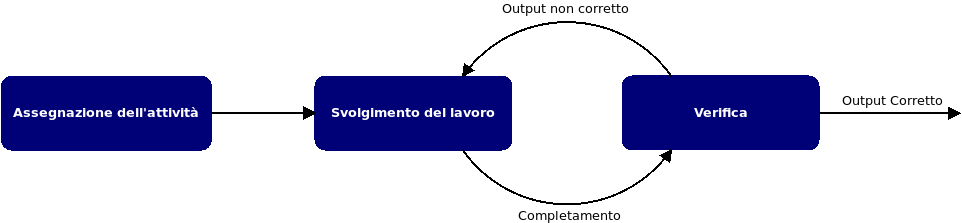
\includegraphics[scale=0.45]{images/Model/activity.png}
	\caption{Ciclo di un'attività}
\end{figure}

		\newpage	

	\section{Pianificazione}
		Per la pianificazione, sono stati individuati 4 fasi, scelte in base alle scadenze decise in comune accordo da tutto il gruppo. Ogni fase contiene diverse attività.\\

\noindent Dopo l'esperienza della fase 1, il gruppo ha pensato di ripianificare le successive fasi, rendendosi conto di aver valutato in maniera non efficiente la ripartizione di costi e risorse. In seguito alla decisione di ripianificare le attività, questa sezione è stata modificata in contenuto e struttura, fatta eccezione per la pianificazione della fase 1 il cui contenuto è rimasto invariato, in quanto già terminata. 
\subsection{Fase 1: Avvio e Analisi dei requisiti (2018-12-04 - 2019-01-21)}
		\subsubsection{Periodo di Avvio (2018-12-04 - 2018-12-17)}
		Nel periodo di avvio hanno luogo le seguenti attività:
		\begin{itemize}
			\item ricerca degli strumenti: tutti i membri del gruppo effettuano le ricerche sui possibili strumenti utili alle attività di avvio e di analisi dei requisiti;
			\item prima normazione: gli amministratori redigono le \textit{NormeDiProgetto\_v2.0.0} concordate per i processi di supporto e organizzativi;
			\item studio di fattibilità: gli analisti redigono lo \textit{StudioDiFattibilità\_v2.0.0} dei capitolati;
			\item pianificazione di progetto: il responsabile redige il \textit{PianoDiProgetto\_v2.0.0}, riportando modello di sviluppo, analisi dei rischi e la pianificazione per le prime attività dell'analisi dei requisiti;
			\item verifica dei documenti: i verificatori controllano che i documenti siano corretti.
		\end{itemize}
		
	\subsubsection{Periodo di Analisi dei Requisiti (2018-12-18 - 2019-01-21)}	
 Il periodo di analisi dei requisiti inizia con le attività di:
			\begin{itemize}
				\item pianificazione di progetto: il responsabile effettua il resoconto del periodo di avvio e pianifica in maniera più dettagliata le attività di analisi dei requisiti; 
				\item pianificazione della qualifica: i verificatori redigono il resoconto del periodo di avvio e gli amministratori effettuano i primi incrementi per il \textit{PianoDiQualifica\_v2.0.0};
				\item normazione: gli amministratori redigono in maniera precisa e completa le \textit{Norme di progetto} per l'attività di analisi;
				\item verifica dei documenti: si procede con la verifica del \textit{PianoDiProgetto\_v2.0.0}, del \textit{PianoDiQualifica\_v2.0.0} e delle \textit{NormeDiProgetto\_v2.0.0}.
				\item analisi dei requisiti del sistema: gli analisti svolgono la prima analisi dei requisiti del sistema;
				\item incrementi al \textit{PianoDiQualifica\_v2.0.0}: i verificatori introducono nel piano i test di sistema in base a quanto scaturito dall'analisi dei requisiti;
				\item verifica dell'analisi dei requisiti di sistema;
				\item incrementi all'analisi dei requisiti: gli analisti aggiungono degli incrementi all'analisi di sistema;
				\item verifica degli incrementi all'analisi dei requisiti;
				\item incrementi al \textit{PianoDiProgetto\_v2.0.0}: il responsabile redige la parte di rendicontazione e consuntivo del \textit{PianoDiProgetto\_v2.0.0} da presentare alla Revisione dei Requisiti.
				\item incrementi al \textit{Piano di qualifica}: i verificatori redigono la parte di rendicontazione del \textit{PianoDiQualifica\_v2.0.0} da presentare alla Revisione dei Requisiti, aggiungendo i risultati delle misurazioni effettuate, e gli analisti aggiungono i restanti test di sistema;
				\item verifica del \textit{PianoDiProgetto\_v2.0.0} e del \textit{PianoDiQualifica\_v2.0.0};
				\item approvazione dei documenti da parte del responsabile;
				\item preparazione alla presentazione.			
			\end{itemize}
			
\begin{figure}[h]
	\centering
	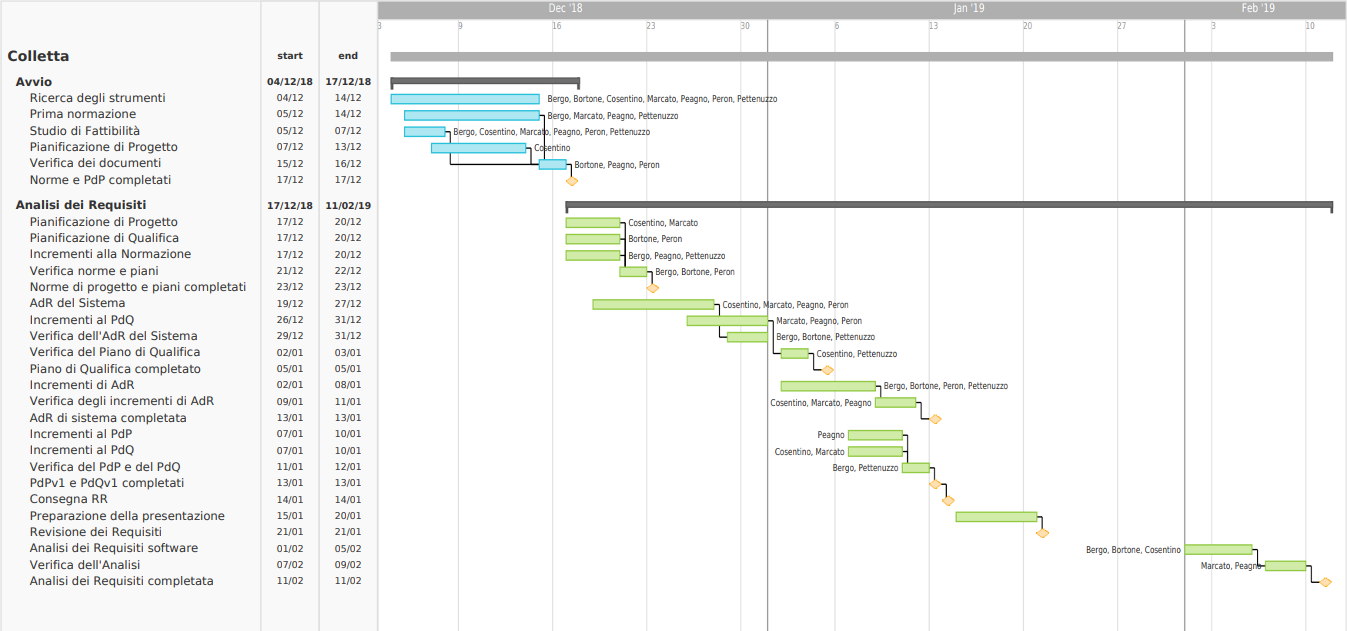
\includegraphics[scale=0.33]{images/ganttan.png}
	\caption{Diagramma di Gantt riguardante la fase 1}
\end{figure}

\subsection{Fase 2: Progettazione della base tecnologica (2019-01-22 - 2019-03-15)}	
	Nella fase 2 si svolgeranno le seguenti attività:
\begin{itemize}
	\item normazione: modifiche alle \textit{Norme di progetto} secondo quanto segnalato alla Revisione dei requisiti. Si procede poi con il suo incremento;
	\item pianificazione della qualifica: modifiche al \textit{Piano di qualifica} secondo quanto segnalato alla Revisione dei requisiti. Si procede poi con il suo incremento;
	\item pianificazione delle attività: modifiche al \textit{Piano di progetto} secondo quanto segnalato alla Revisione dei requisiti;
	\item analisi dei requisiti: modifiche al \textit{Analisi dei requisiti} secondo quanto segnalato alla Revisione dei requisiti;
	\item progettazione PoC e Technology Baseline: vengono ricercate le tecnologie, i framework e le librerie ritenute più adatte allo sviluppo del prodotto;
	\item codifica: realizzazione del PoC;
	\item verifica per il colloquio: verifica del PoC in vista di una discussione Agile con il committente;
	\item colloquio: viene effettuato il colloquio con la committente;
	\item incremento progettazione e codifica: in base alla segnalazioni ricevute durante il colloquio con il committente vengono eseguite opportune modifiche;
	\item incremento della pianificazione delle attività: viene aggiornato il \textit{Piano di progetto} con il consuntivo riguardante la fase 2;
	\item verifica per la consegna: vengono verificati tutti i documenti e la Technology Baseline con la relativa codifica;
	\item consegna del materiale in ingresso;
	\item preparazione alla presentazione.
\end{itemize}

\begin{figure}[h]
	\centering
	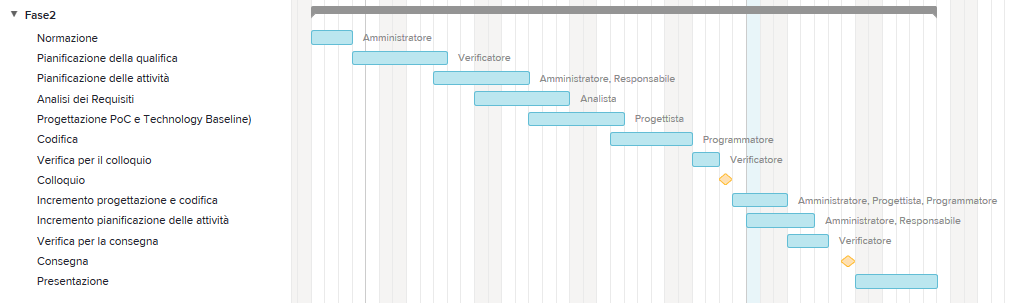
\includegraphics[scale=0.67]{images/fase2.png}
	\caption{Diagramma di Gantt riguardante la fase 2}
\end{figure}
	
\subsection{Fase 3: Progettazione di dettaglio e codifica (2019-03-16 - 2019-04-19)}
	Nella fase 3 hanno luogo le seguenti attività:
\begin{itemize}
	\item normazione: modifiche alle \textit{NormeDiProgetto\_v2.0.0} secondo quanto segnalato alla Revisione di progettazione. Si procede poi con il suo incremento;
	\item pianificazione della qualifica: modifiche al \textit{PianoDiQualifica\_v2.0.0} secondo quanto segnalato alla Revisione di Progettazione. Si procede poi con il suo incremento;
	\item pianificazione delle attività: modifiche al \textit{PianoDiProgetto\_v2.0.0} secondo quanto segnalato alla Revisione di progettazione;
	\item progettazione in dettaglio e Product Baseline: questa attività consiste nella progettazione del prodotto tramite diagrammi delle classi e di sequenza, incrementando quanto sviluppato nel PoC.
	\item codifica: realizzazione del prodotto;
	\item verifica per il colloquio: verifica del codice scritto in vista del colloquio Agile con il committente;
	\item colloquio: viene effettuato il colloquio con il committente;
	\item redazione manuali: redazione \textit{Manuale Utente} e \textit{Manuale Sviluppatore};
	\item incremento progettazione e codifica: in base alle segnalazioni ricevute al colloquio con il committente viene eseguito l'eventuale incremento;
	\item incremento della pianificazione delle attività: viene aggiornato il \textit{Piano di Progetto} con il consuntivo pre-finale;
	\item verifica per la consegna: vengono verificati tutti i documenti e il Product Baseline con la relativa codifica;
	\item approvazione dei documenti da parte del responsabile. Sono pronti per il rilascio le \textit{NormeDiProgetto\_v3.0.0}, il \textit{PianoDiProgetto\_v3.0.0}, il \textit{PianoDiQualifica\_v3.0.0}, l'\textit{AnalisiDeiRequisiti\_v3.0.0}, il
	\textit{ManualeUtente\_v1.0.0} e il \textit{ManualeSviluppatore\_v1.0.0}
	\item preparazione alla presentazione.
\end{itemize}

\begin{figure}[h]
	\centering
	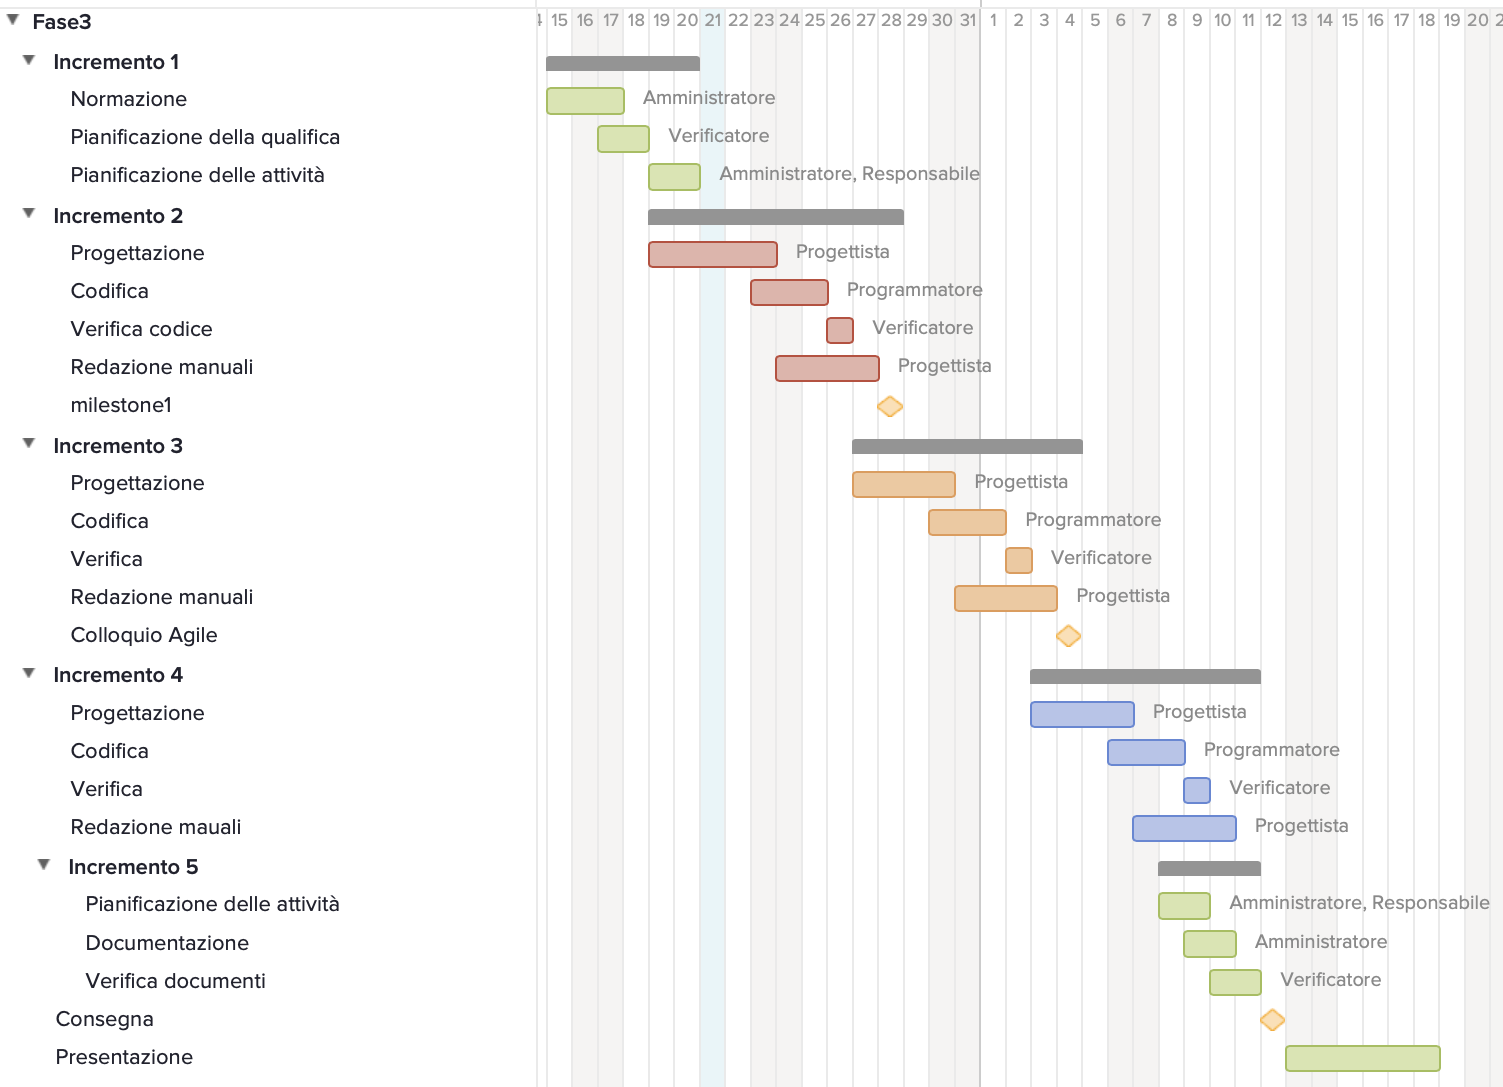
\includegraphics[scale=0.70]{images/fase3.png}
	\caption{Diagramma di Gantt riguardante la fase 3}
\end{figure}
	
\subsection{Fase 4: Validazione e collaudo (2019-04-21 - 2019-05-17)}
	Nella fase 4 vengono eseguite le seguenti attività:
\begin{itemize}
	\item normazione: modifiche alle \textit{Norme di progetto} secondo quanto segnalato alla Revisione dei requisiti. Si procede poi con il suo incremento;
	\item pianificazione della qualifica: modifiche al \textit{PianoDiQualifica\_v2.0.0} secondo quanto segnalato alla Revisione di qualifica; Si procede poi con il suo incremento;
	\item pianificazione delle attività: modifiche al \textit{PianoDiProgetto\_v2.0.0} secondo quanto segnalato alla Revisione di qualifica;
	\item progettazione di dettaglio: incremento al \textit{Product Baseline} con secondo quanto segnalato alla Recisione di qualifica;
	\item codifica: codifica degli incrementi effettuati durante la progettazione;
	\item redazione manuali: incrementi al \textit{ManualeUtente\_v2.0.0} e al \textit{ManualeSviluppatore\_v2.0.0} in base a quanto segnalato alla Revisione di qualifica;
	\item verifica: verifica degli incrementi effettuati;
	\item validazione e collaudo: vengono eseguiti i test di qualifica e il collaudo per il rilascio;
	\item preparazione alla presentazione;
	\item consegna del materiale in ingresso.
\end{itemize}

\begin{figure}[h]
	\centering
	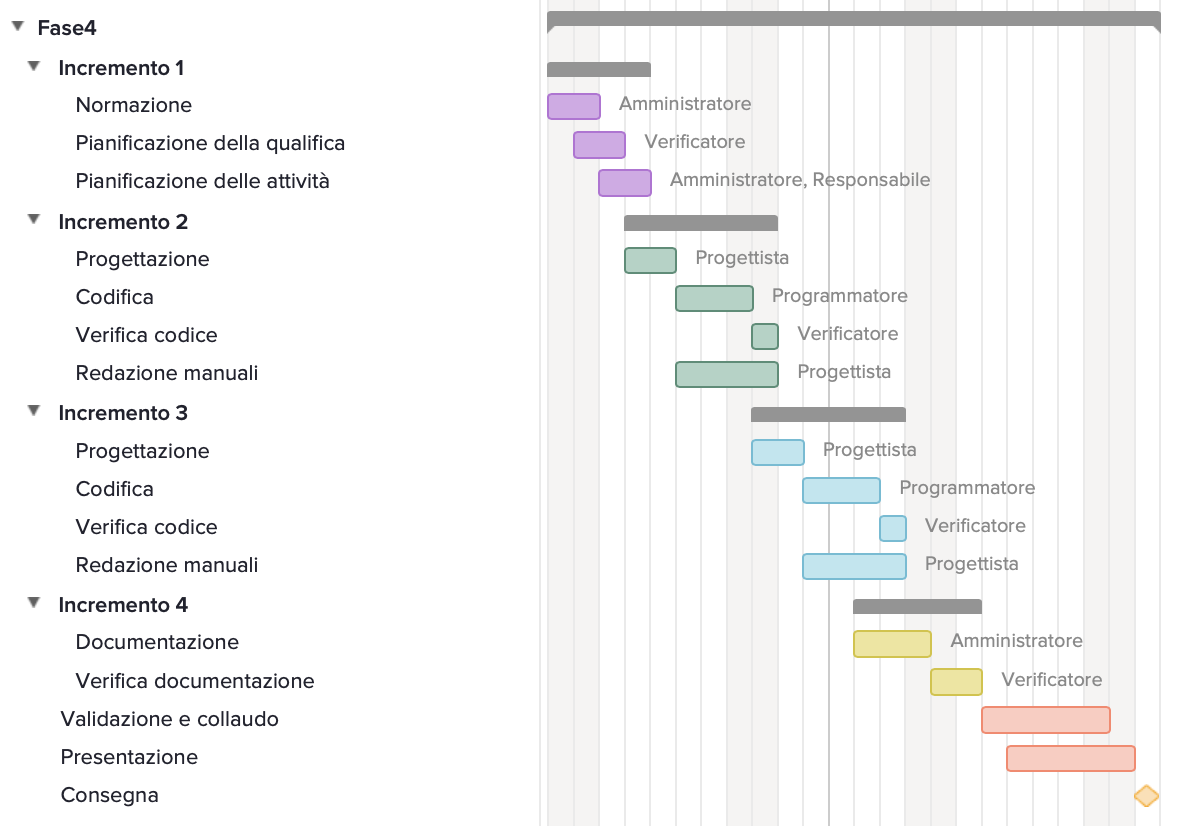
\includegraphics[scale=0.70]{images/fase4.png}
	\caption{Diagramma di Gantt riguardante la fase 4}
\end{figure}
	
\newpage
		
	\section{Preventivo}
%		In questa sezione, vengono riportati il preventivo per ogni periodo del progetto e i dati utili a ricavarlo. Il preventivo definisce il budget e quindi il costo totale del progetto. Ogni tabella fa riferimento a una specifica fase del progetto (indicata con un numero sequenziale) che parte da una determinata data a un'altra.
Le fasi individuate corrispondono agli intervalli tra una revisione e l'altra e, nel caso della fase 1, all'intervallo di tempo che parte dall'inizio del progetto fino alla Revisione dei Requisiti. In particolare,
\begin{enumerate}
	\item Fase 1 (2018-12-04 - 2019-01-21); 
	\item Fase 2 (2019-01-22 - 2019-03-15);
	\item Fase 3 (2019-03-16 - 2019-04-19);
	\item Fase 4 (2019-04-20 - 2019-05-17).
\end{enumerate}
Per ogni fase sono presenti: un prospetto orario che indica le ore preventivate per ciascun membro e per ciascun ruolo, una tabella dei costi per membro e una tabella dei costi per ruolo.\\
Per indicare i ruoli, sono state impiegate le seguenti abbreviazioni:
\begin{itemize}
	\item RES: responsabile;
	\item AMM: amministratore;
	\item AN: analista;
	\item PRO: progettista;
	\item DEV: programmatore;
	\item VER: verificatore.
\end{itemize}

\newpage
\subsection{Fase 1 (2018-12-04 - 2019-01-21)}
	Le ore di questo periodo vanno considerate come investimento e non rientrano nelle ore da rendicontare per il preventivo.
	\subsubsection{Ore preventivate}
		La seguente tabella indica le ore di lavoro per ciascun membro e per ciascun ruolo:
		\begin{table}[h]
			\centering
			\begin{tabular}{| l | c c c c c c | c |}
				\rowcolor{LightBlue}
				& \multicolumn{7}{c}{\textbf{\color{white}Numero di ore}}	\\
	
				\rowcolor{LightBlue}
				\textbf{\color{white}Membro}
				& \textbf{\color{white}RES}
				& \textbf{\color{white}AMM}
				& \textbf{\color{white}AN}
				& \textbf{\color{white}PRO}
				& \textbf{\color{white}DEV}
				& \textbf{\color{white}VER}
				& \textbf{\color{white}Totali}\\
	
				Bergo 				& - & 15 & 14 & - & - & 8 & 37\\
				Bortone 			& - & 10 & 15	& - & - & 8 & 33\\
				Cosentino 		& 20 & - & 22 & - & - & 5 & 47\\
				Marcato 			& 5 & 10 & 25 & - & - & 3 & 43\\
				Peagno 			& 5 & 15 & 22 & - & - & 3 & 45\\
				Peron 				& - & 10 & 29 & - & - & 5 & 44\\
				Pettenuzzo 	& - & 15 & 19 & - & - & 5 & 39\\ \hline
			\end{tabular}
			\caption{Ore di lavoro per membro/ruolo della fase 1}
		\end{table}
		
				\begin{figure}[h]
	\centering
	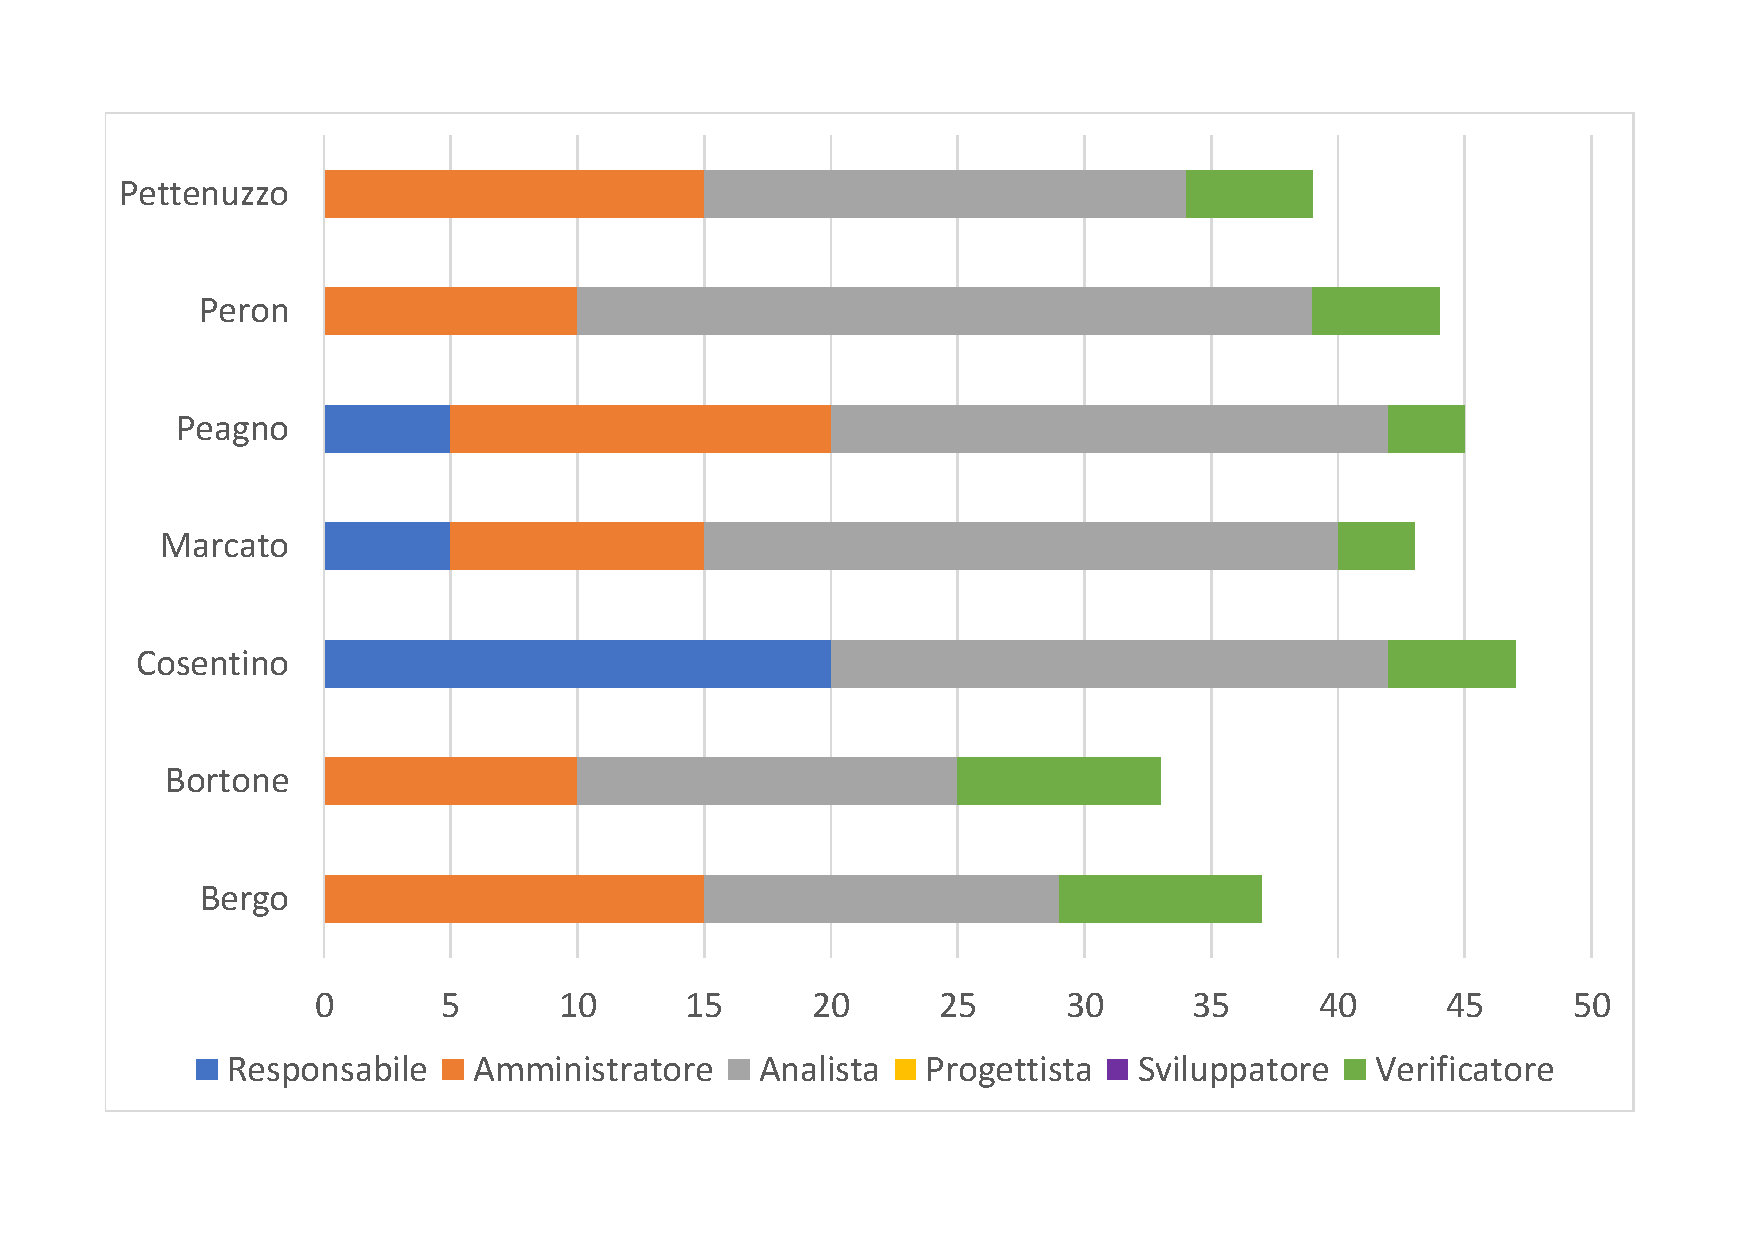
\includegraphics[scale=0.45]{images/preventivoRR.pdf}
	\caption{}
\end{figure}
		
	\subsubsection{Costo}
		Le seguenti tabelle indicano i costi in base ai membri e in base ai ruoli:
		\begin{table}[h]
			\centering		
			\begin{tabular}{| l | l |}
				\rowcolor{LightBlue}
				\textbf{\color{white}Membro}
				& \textbf{\color{white}Costo}\\
			
				Bergo 				& 770€\\
				Bortone 			& 695€\\
				Cosentino 		& 1225€\\
				Marcato 			& 1020€\\
				Peagno 			& 1045€\\
				Peron 				& 1000€\\
				Pettenuzzo 	& 850€\\ \hline
				\textbf{Totale} & 6605€\\ \hline
			\end{tabular}
			\caption{Costo di ciascun membro nella fase 1}
		\end{table}
		
		\begin{table}[h]
			\centering		
			\begin{tabular}{| l | l |}
				\rowcolor{LightBlue}
				\textbf{\color{white}Ruolo}
				& \textbf{\color{white}Costo}\\
			
				Responsabile 		& 900€\\
				Amministratore 	& 1500€\\
				Analista 				& 3650€\\			
				Progettista 			& 0€\\
				Programmatore 		& 0€\\
				Verificatore 		& 555€\\ \hline
				\textbf{Totale} 	& 6605€\\ \hline
			\end{tabular}
			\caption{Costo di ciascun ruolo nella fase 1}
		\end{table}
		

\newpage
\subsection{Fase 2 (2019-01-22 - 2019-03-15)}
	\subsubsection{Ore preventivate}
		La seguente tabella indica le ore di lavoro per ciascun membro e per ciascun ruolo:
		\begin{table}[h]
			\centering
			\begin{tabular}{| l | c c c c c c | c |}
				\rowcolor{LightBlue}
				& \multicolumn{7}{c}{\textbf{\color{white}Numero di ore}}	\\
	
				\rowcolor{LightBlue}
				\textbf{\color{white}Membro}
				& \textbf{\color{white}RES}
				& \textbf{\color{white}AMM}
				& \textbf{\color{white}AN}
				& \textbf{\color{white}PRO}
				& \textbf{\color{white}DEV}
				& \textbf{\color{white}VER}
				& \textbf{\color{white}Totali}\\

				Bergo      & - & 5 & - & 15 & 15 & 5 	& 40 \\
				Bortone    & - & - & - & 21 & 14 & - & 35 \\
				Cosentino  & - & - & 5 & 13 & 5 & 5 & 28 \\
				Marcato    & - & 10 & - & 10 & 7 & 5 & 32 \\
				Peagno     & - & 4 & - & 16 & - & 10 & 30 \\
				Peron      & 15 & - & - & 10 & 10 & - & 35 \\
				Pettenuzzo & 15 & - & 10 & 5 & - & - & 30 \\ \hline
			\end{tabular}
			\caption{Ore di lavoro per membro/ruolo della fase 2}
		\end{table}	
				\begin{figure}[h]
	\centering
	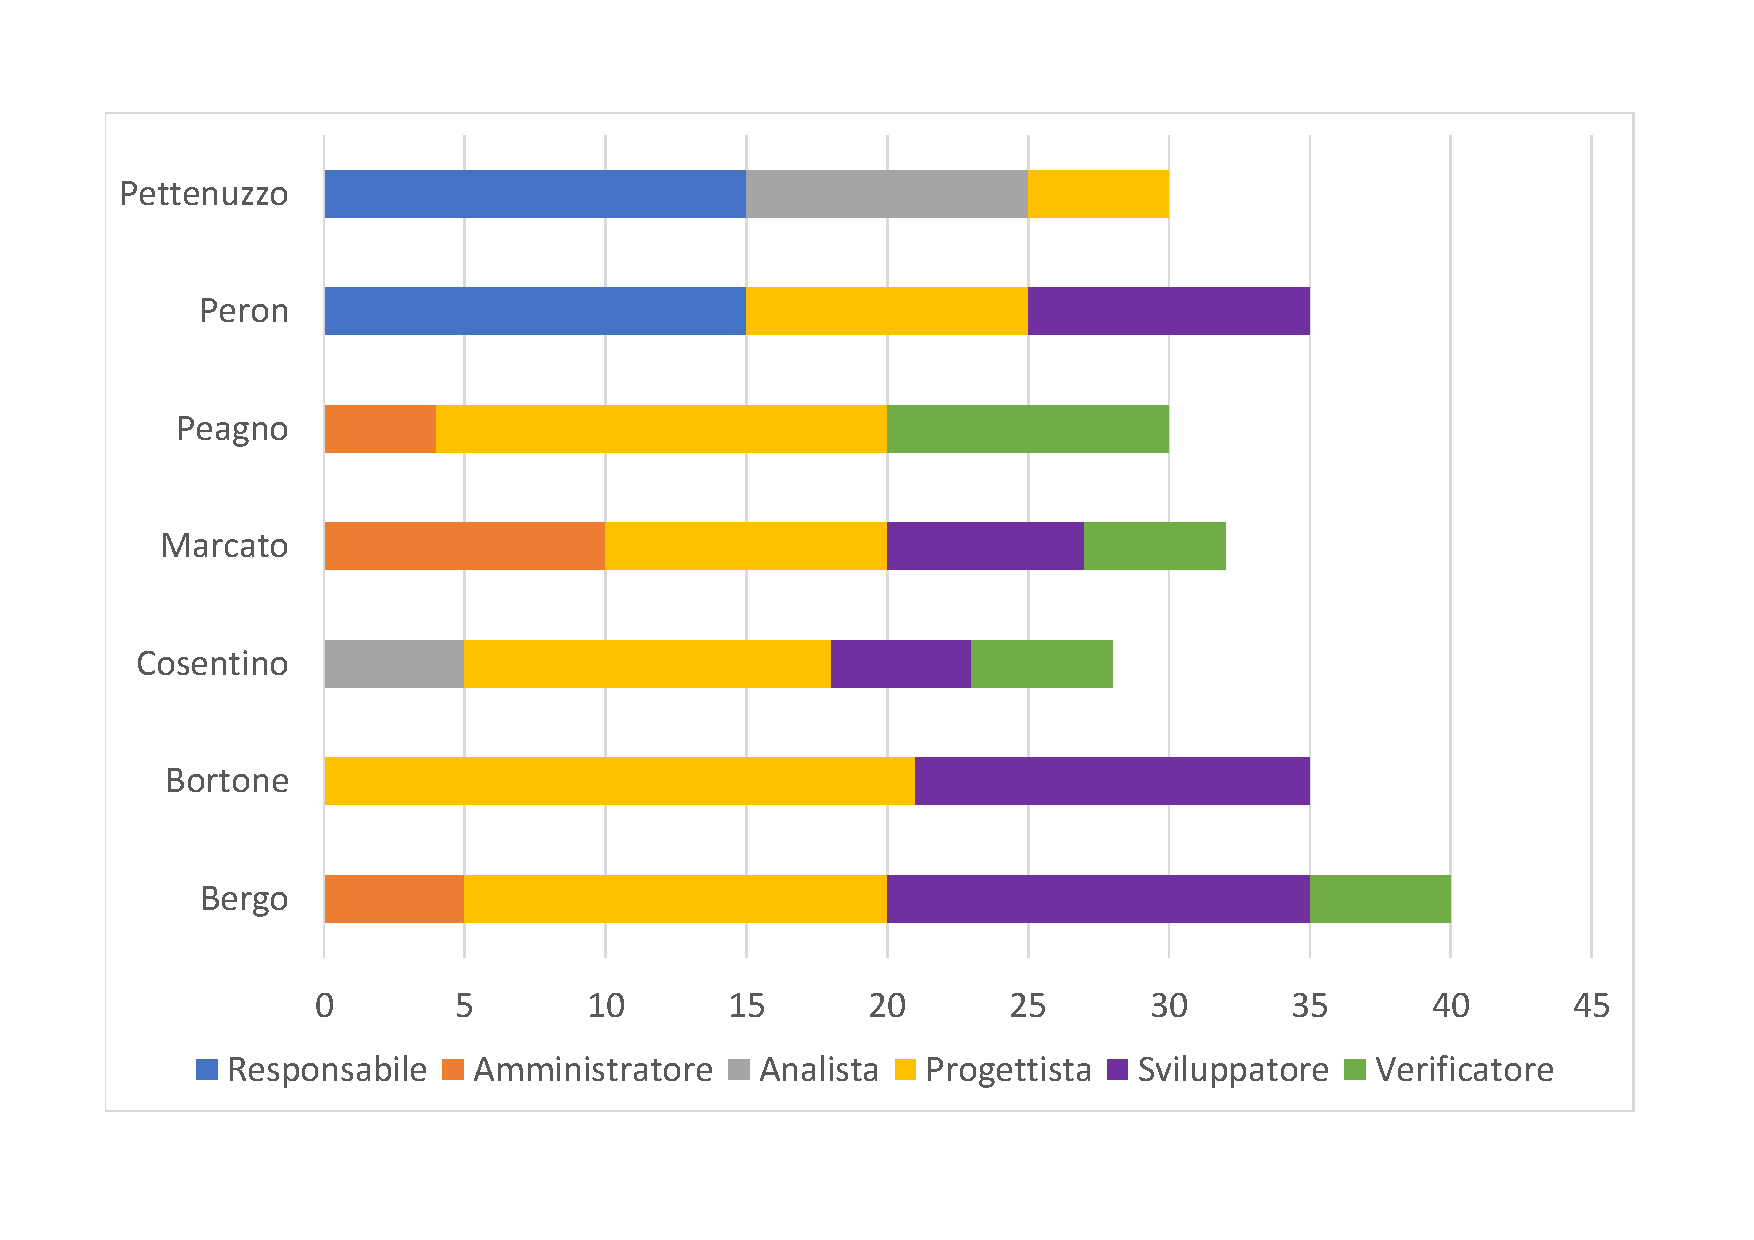
\includegraphics[scale=0.45]{images/preventivoRP.pdf}
	\caption{}
\end{figure}	
		
	\subsubsection{Costo}
		Le seguenti tabelle indicano i costi in base ai membri e in base ai ruoli:	
		\begin{table}[h]
			\centering
			\begin{tabular}{| l | l |}
				\rowcolor{LightBlue}
				\textbf{\color{white}Membro}
				& \textbf{\color{white}Costo}\\
			
				Bergo				& 730€\\
				Bortone			& 672€\\
				Cosentino		& 561€\\
				Marcato			& 600€\\
				Peagno				& 582€\\
				Peron				& 820€\\
				Pettenuzzo		& 810€\\ \hline
				\textbf{Totale} & 4775€\\ \hline
			\end{tabular}
			\caption{Costo di ciascun membro nella fase 2}
		\end{table}
		
		\begin{table}[h]
			\centering
			\begin{tabular}{| l | l |}
				\rowcolor{LightBlue}
				\textbf{\color{white}Ruolo}
				& \textbf{\color{white}Costo}\\
			
				Responsabile 		& 900€\\
				Amministratore 	& 380€\\
				Analista 				& 375€\\			
				Progettista 			& 1980€\\
				Programmatore 		& 765€\\
				Verificatore 		& 375€\\ \hline
				\textbf{Totale} 	& 4775€\\ \hline
			\end{tabular}		
			\caption{Costo di ciascun ruolo nella fase 2}
		\end{table}
		
\newpage
\subsection{Fase 3 (2019-03-16 - 2019-04-19)}
	\subsubsection{Ore preventivate}
		La seguente tabella indica le ore di lavoro per ciascun membro e per ciascun ruolo:
		\begin{table}[h]
			\centering
			\begin{tabular}{| l | c c c c c c | c |}
				\rowcolor{LightBlue}
				& \multicolumn{7}{c}{\textbf{\color{white}Numero di ore}}	\\
	
				\rowcolor{LightBlue}
				\textbf{\color{white}Membro}
				& \textbf{\color{white}RES}
				& \textbf{\color{white}AMM}
				& \textbf{\color{white}AN}
				& \textbf{\color{white}PRO}
				& \textbf{\color{white}DEV}
				& \textbf{\color{white}VER}
				& \textbf{\color{white}Totali}\\
	
				Bergo      & 15 & - & - & 10 & 10 & 10 & 45 \\
				Bortone    & 15 & - & 5 & 8 & 7 & 10 & 45  \\
				Cosentino  & - & 5 & - & 21 & 21 & - & 47 \\
				Marcato    & - & - & - & 25 & 25 & - & 50 \\
				Peagno     & - & - & - & 25 & 25 & - & 50 \\
				Peron      & - & - & - & 15 & 15 & 15 & 45 \\
				Pettenuzzo & - & - & 5 & 10 & 25 & 10 & 50 \\ \hline
			\end{tabular}
			\caption{Ore di lavoro per membro/ruolo della fase 3}
		\end{table}
		
				\begin{figure}[h]
	\centering
	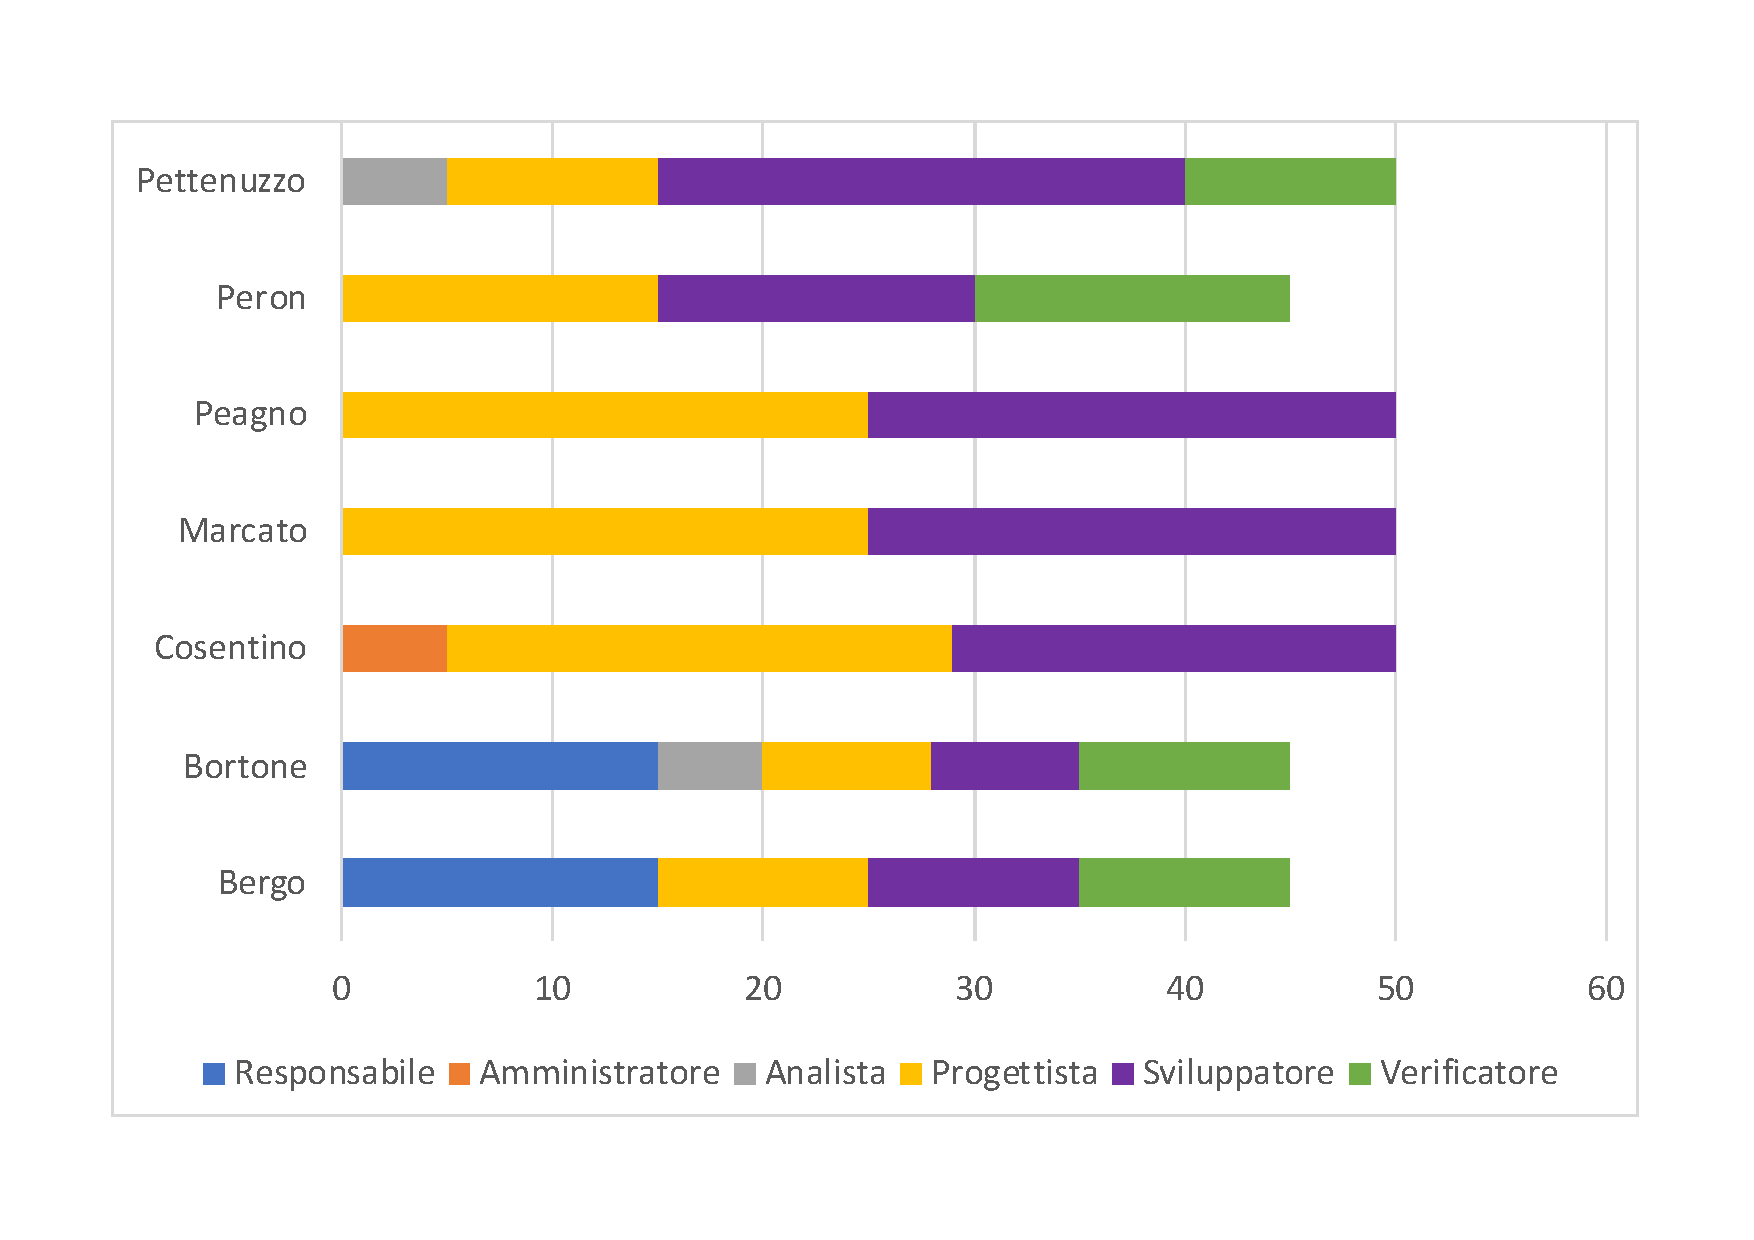
\includegraphics[scale=0.45]{images/preventivoRQ.pdf}
	\caption{}
\end{figure}

	\subsubsection{Costo}
		Le seguenti tabelle indicano i costi in base ai membri e in base ai ruoli:
		\begin{table}[h]
			\centering
			\begin{tabular}{| l | l |}
				\rowcolor{LightBlue}
				\textbf{\color{white}Membro}
				& \textbf{\color{white}Costo}\\
				
				Bergo 				& 970€\\
				Bortone 			& 1006€\\
				Cosentino 		& 877€\\
				Marcato 			& 925€\\
				Peagno 			& 925€\\
				Peron 				& 780€\\
				Pettenuzzo 	& 870€\\ \hline
				\textbf{Totale} & 6353€\\ \hline
			\end{tabular}
			\caption{Costo di ciascun membro nella fase 3}
		\end{table}
		
		\begin{table}[h]
			\centering
			\begin{tabular}{| l | l |}
				\rowcolor{LightBlue}
				\textbf{\color{white}Ruolo}
				& \textbf{\color{white}Costo}\\
				
				Responsabile 		& 900€\\
				Amministratore 	& 100€\\
				Analista 				& 250€\\			
				Progettista 			& 2508€\\
				Programmatore 		& 1920€\\
				Verificatore 		& 675€\\ \hline
				\textbf{Totale} 	& 6353€\\ \hline
			\end{tabular}
			\caption{Costo di ciascun ruolo nella fase 3}
		\end{table}
		
\newpage
\subsection{Fase 4 (2019-04-20 - 2019-05-17)}
	\subsubsection{Ore preventivate}
		La seguente tabella indica le ore di lavoro per ciascun membro e per ciascun ruolo:
		\begin{table}[h]
			\centering
			\begin{tabular}{| l | c c c c c c | c |}
				\rowcolor{LightBlue}
				& \multicolumn{7}{c}{\textbf{\color{white}Numero di ore}}	\\
		
				\rowcolor{LightBlue}
				\textbf{\color{white}Membro}
				& \textbf{\color{white}RES}
				& \textbf{\color{white}AMM}
				& \textbf{\color{white}AN}
				& \textbf{\color{white}PRO}
				& \textbf{\color{white}DEV}
				& \textbf{\color{white}VER}
				& \textbf{\color{white}Totali}\\
	
				Bergo      & - & - & - & 11 & 11 & - & 22\\
				Bortone    & - & - & - & 8 & 8 & 8 & 24\\
				Cosentino  & - & 3 & - & 7 & 7 & 10 & 27\\
				Marcato    & - & - & - & - & 9 & 10 & 19\\
				Peagno     & 15 & - & - & - & 10 & - & 25\\
				Peron      & - & - & - & 5 & 10 & 10 & 25\\
				Pettenuzzo & - & - & - & 15 & - & 8 & 23\\ \hline
			\end{tabular}
			\caption{Ore di lavoro per membro/ruolo della fase 4}
		\end{table}
		
				\begin{figure}[h]
	\centering
	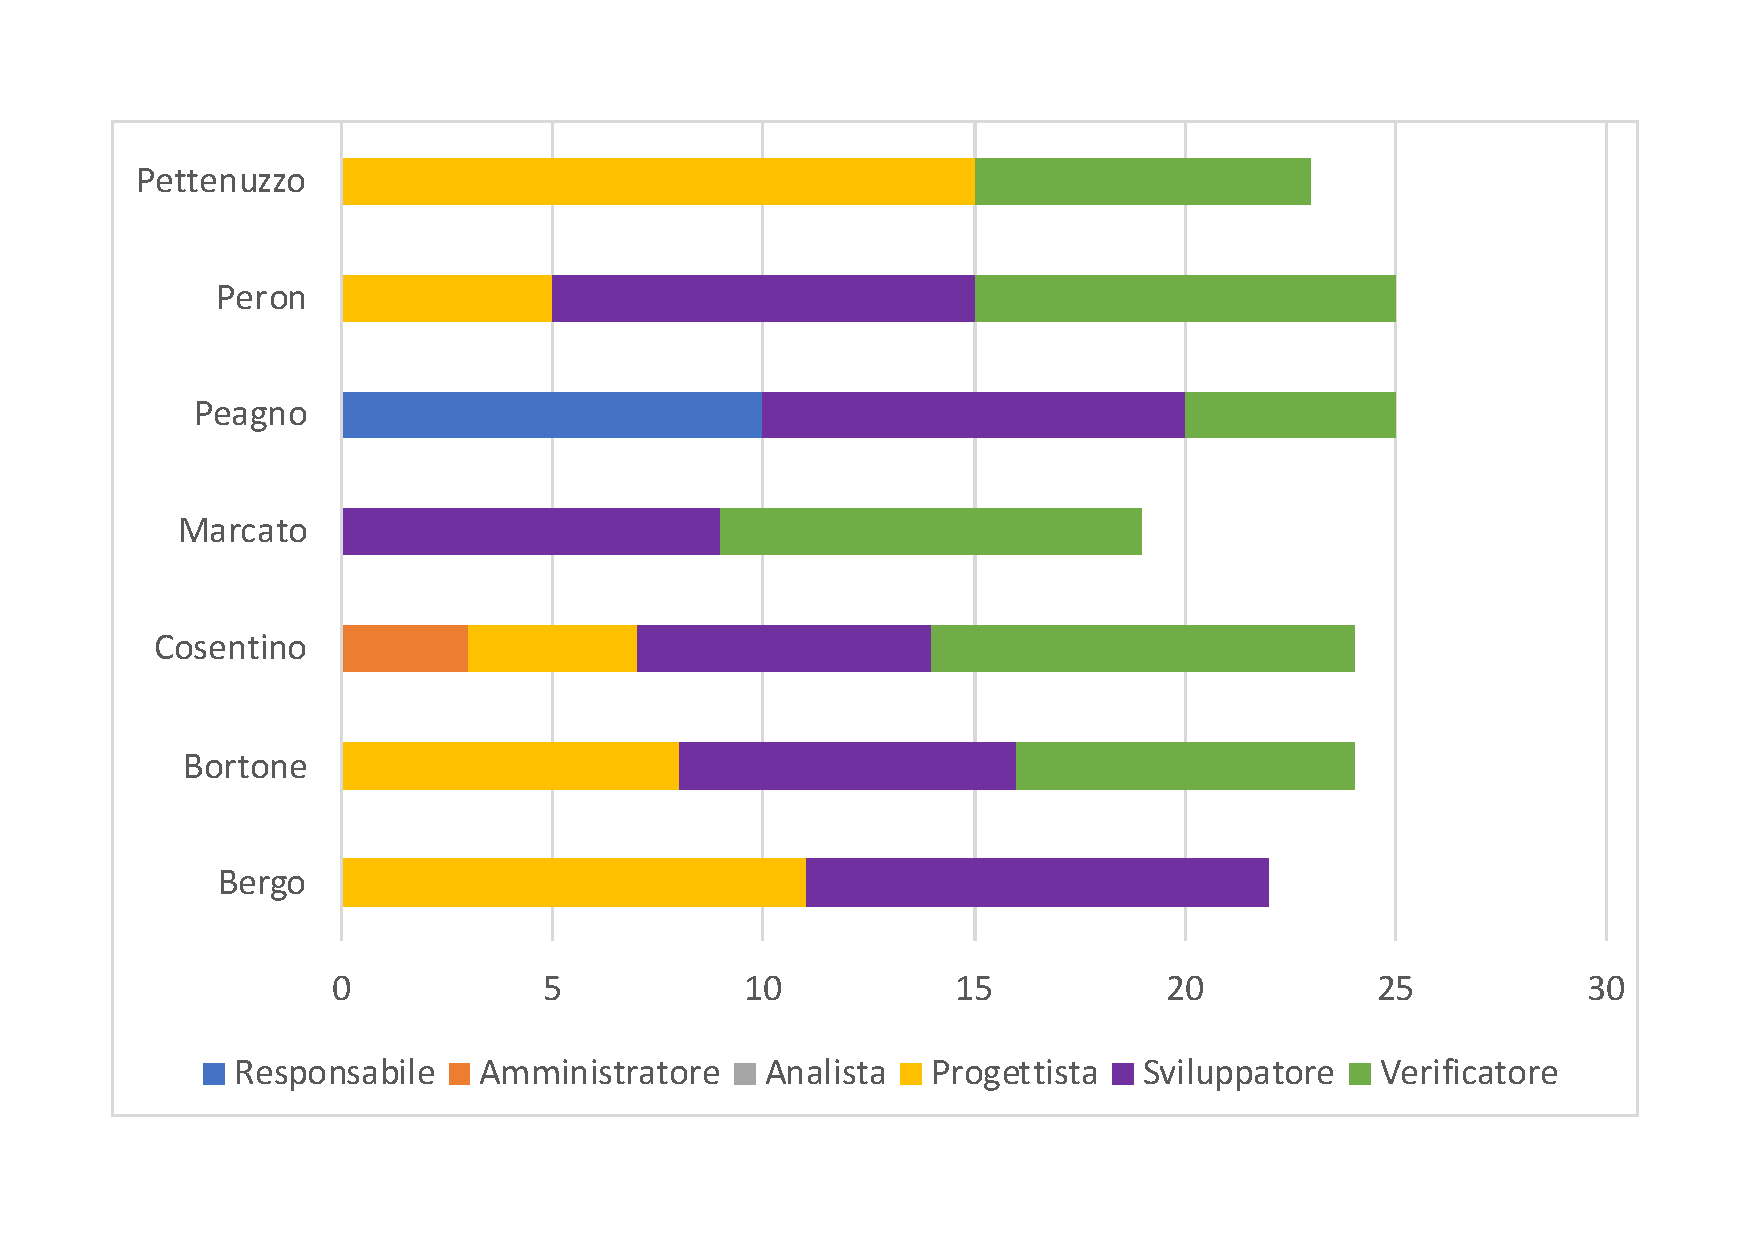
\includegraphics[scale=0.45]{images/preventivoRA.pdf}
	\caption{}
\end{figure}
		
	\subsubsection{Costo}
		Le seguenti tabelle indicano i costi in base ai membri e in base ai ruoli:
		\begin{table}[h]
			\centering
			\begin{tabular}{| l | l |}
				\rowcolor{LightBlue}
				\textbf{\color{white}Membro}
				& \textbf{\color{white}Costo}\\
				
				Bergo				& 407€\\
				Bortone			& 416€\\
				Cosentino		& 469€\\
				Marcato			& 285€\\
				Peagno				& 600€\\
				Peron				& 410€\\
				Pettenuzzo		& 450€\\ \hline
				\textbf{Totale} & 3037€\\ \hline
			\end{tabular}
			\caption{Costo di ciascun membro nella fase 4}
		\end{table}
		
		\begin{table}[h]
			\centering
			\begin{tabular}{| l | l |}
				\rowcolor{LightBlue}
				\textbf{\color{white}Ruolo}
				& \textbf{\color{white}Costo}\\
				
				Responsabile 		& 450€\\
				Amministratore 	& 60€\\
				Analista 				& 0€\\			
				Progettista 			& 1012€\\
				Programmatore 		& 825€\\
				Verificatore 		& 690€\\ \hline
				\textbf{Totale} 	& 3037€\\ \hline
			\end{tabular}		
			\caption{Costo di ciascun ruolo nella fase 4}
		\end{table}

\newpage
\subsection{Riepilogo}
	\subsubsection{Ore totali}
		La seguente tabella indica le ore di lavoro per ciascun membro e per ciascun ruolo. Tra parentesi vengono indicate le ore totali considerando anche l'investimento. Le ore rendicontate sono quelle delle fasi 2, 3 e 4. La fase 1 è da considerare come investimento per il progetto.
		\begin{table}[h]
			\centering
			\begin{tabular}{| l | c c c c c c | c |}
				\rowcolor{LightBlue}
				& \multicolumn{7}{c}{\textbf{\color{white}Numero di ore}}	\\
		
				\rowcolor{LightBlue}
				\textbf{\color{white}Membro}
				& \textbf{\color{white}RES}
				& \textbf{\color{white}AMM}
				& \textbf{\color{white}AN}
				& \textbf{\color{white}PRO}
				& \textbf{\color{white}DEV}
				& \textbf{\color{white}VER}
				& \textbf{\color{white}Totali}\\
		
				Bergo 				& 15 (15) & 5 (20)		& 0 (14)	& 36 (36) & 36 (36) & 10 (18)	& 102 (139)\\
				Bortone 			& 15  (15)  & 0 (10)		& 5	 (20)	& 37 (37) & 29 (29) & 18 (26)	& 104 (137)\\
				Cosentino 		& 0  (20) & 8 (8)		& 5 (27)	& 41 (41) & 33 (33) & 15  (20)	& 102 (149)\\
				Marcato 			& 0 (5) & 10 (20)		& 0  (25)	& 35 (35) & 41 (41) & 15 (18)	& 101 (144)\\
				Peagno 			& 15  (20) & 4 (19)		& 0  (22)	& 41 (41) & 35 (35) & 10 (13)	& 105 (150)\\
				Peron 				& 15 (15) & 0 (10)		& 0  (29)	& 30 (30) & 35 (35) & 25  (30)	& 105 (149)\\
				Pettenuzzo 	& 15 (15) & 0 (15) 	& 15  (34)	& 30 (30) & 25 (25) & 18 (23)	& 103 (142)\\ \hline
			\end{tabular}
			\caption{Ore di lavoro per membro/ruolo di tutto il progetto}
		\end{table}
	
	\subsubsection{Costo totale}
		Le seguenti tabelle indicano i costi con e senza investimento in base ai membri e in base ai ruoli.
		\begin{table}[h]
			\centering
			\begin{tabular}{| l | l | l |}
				\rowcolor{LightBlue}
				\textbf{\color{white}Membro}
				& \textbf{\color{white}Costo con investimento}
				& \textbf{\color{white}Costo preventivato}\\
				
				Bergo				& 2802€ & 2032€\\
				Bortone			& 2789€ & 2094€\\
				Cosentino		& 3132€ & 1907€\\
				Marcato			& 2830€ & 1810€\\
				Peagno				& 3152€ & 2107€\\
				Peron				& 3010€ & 2010€\\
				Pettenuzzo		& 2980€ & 2130€\\ \hline
				\textbf{Totale} & 20695€ & 14090€\\ \hline
			\end{tabular}
			\caption{Costo di ciascun membro per tutto il progetto}
		\end{table}
		
		\begin{table}[h]
			\centering
			\begin{tabular}{| l | l | l |}
				\rowcolor{LightBlue}
				\textbf{\color{white}Ruolo}
				& \textbf{\color{white}Costo con investimento}
				& \textbf{\color{white}Costo preventivato}\\
				
				Responsabile 		& 3150€ & 2225€\\
				Amministratore 	& 2040€ & 540€\\
				Analista 				& 4275€ & 625€\\			
				Progettista 			& 5500€ & 5500€\\
				Programmatore 		& 3510€ & 3510€\\
				Verificatore 		& 2220€ & 1665€\\ \hline
				\textbf{Totale} 	& 20695€ & 14090€\\ \hline
			\end{tabular}		
			\caption{Costo di ciascun ruolo per tutto il progetto}
		\end{table}
		
		\paragraph{Conclusioni\\}
		Il costo totale del progetto con un investimento di 6605 è pari a \textbf{20695€}. Conseguentemente, il costo preventivato è \textbf{14090€}.
		
	\section{Consuntivo e preventivo a finire}
%		\subsection{Fase 1 (2018-12-04 - 2019-01-21)}
	\subsubsection{Ore impiegate}
	La seguente tabella indica le ore impiegate durante la fase 1. Tra parentesi viene indicata la differenza tra ore preventivate e ore impiegate ($preventivo - consuntivo$): valori positivi indicano le ore risparmiate e valori negativi indicano le ore in eccesso.
	
	\begin{table}[H]
		\centering
		\begin{tabular}{| l | c c c c c c | c |}
			\rowcolor{LightBlue}
			& \multicolumn{7}{c}{\textbf{\color{white}Numero di ore}}	\\	
			\rowcolor{LightBlue}
			\textbf{\color{white}Membro}
			& \textbf{\color{white}RES}
			& \textbf{\color{white}AMM}
			& \textbf{\color{white}AN}
			& \textbf{\color{white}PRO}
			& \textbf{\color{white}DEV}
			& \textbf{\color{white}VER}
			& \textbf{\color{white}Totali}\\	
			Bergo     		& -  (0)		& 9  (+6) 	& 22 (-8) 		& - (0) & - (0) & 7  (+1) 	& 38\\
			Bortone   		& -  (0)		& 14 (-4) 	& 18 (-3) 		& - (0) & - (0) & 10 (-2)	& 42\\
			Cosentino 		& 25 (-5) 	& -  (0) 	& 24 (-2) 		& - (0) & - (0) & -  (+5)	& 49\\
			Marcato   		& 10 (-5) 	& 10 (0) 	& 22 (+3) 		& - (0) & - (0) & -  (+3)	& 42\\
			Peagno    		& -  (+5) 	& 15 (0) 	& 23 (-1) 		& - (0) & - (0) & -  (+3)	& 38\\
			Peron     		& -  (0)		& 13 (-3) 	& 23 (+6) 		& - (0) & - (0) & 13 (-8)	& 49\\
			Pettenuzzo 	& - (0) 		& 12 (+3) 	& 5  (+14) 	& - (0) & - (0) & 13 (-8)	& 30\\ \hline
		\end{tabular}
		\caption{Ore di lavoro impiegate per membro/ruolo della fase 1}
	\end{table}
	
	\begin{figure}[H]
		\centering
		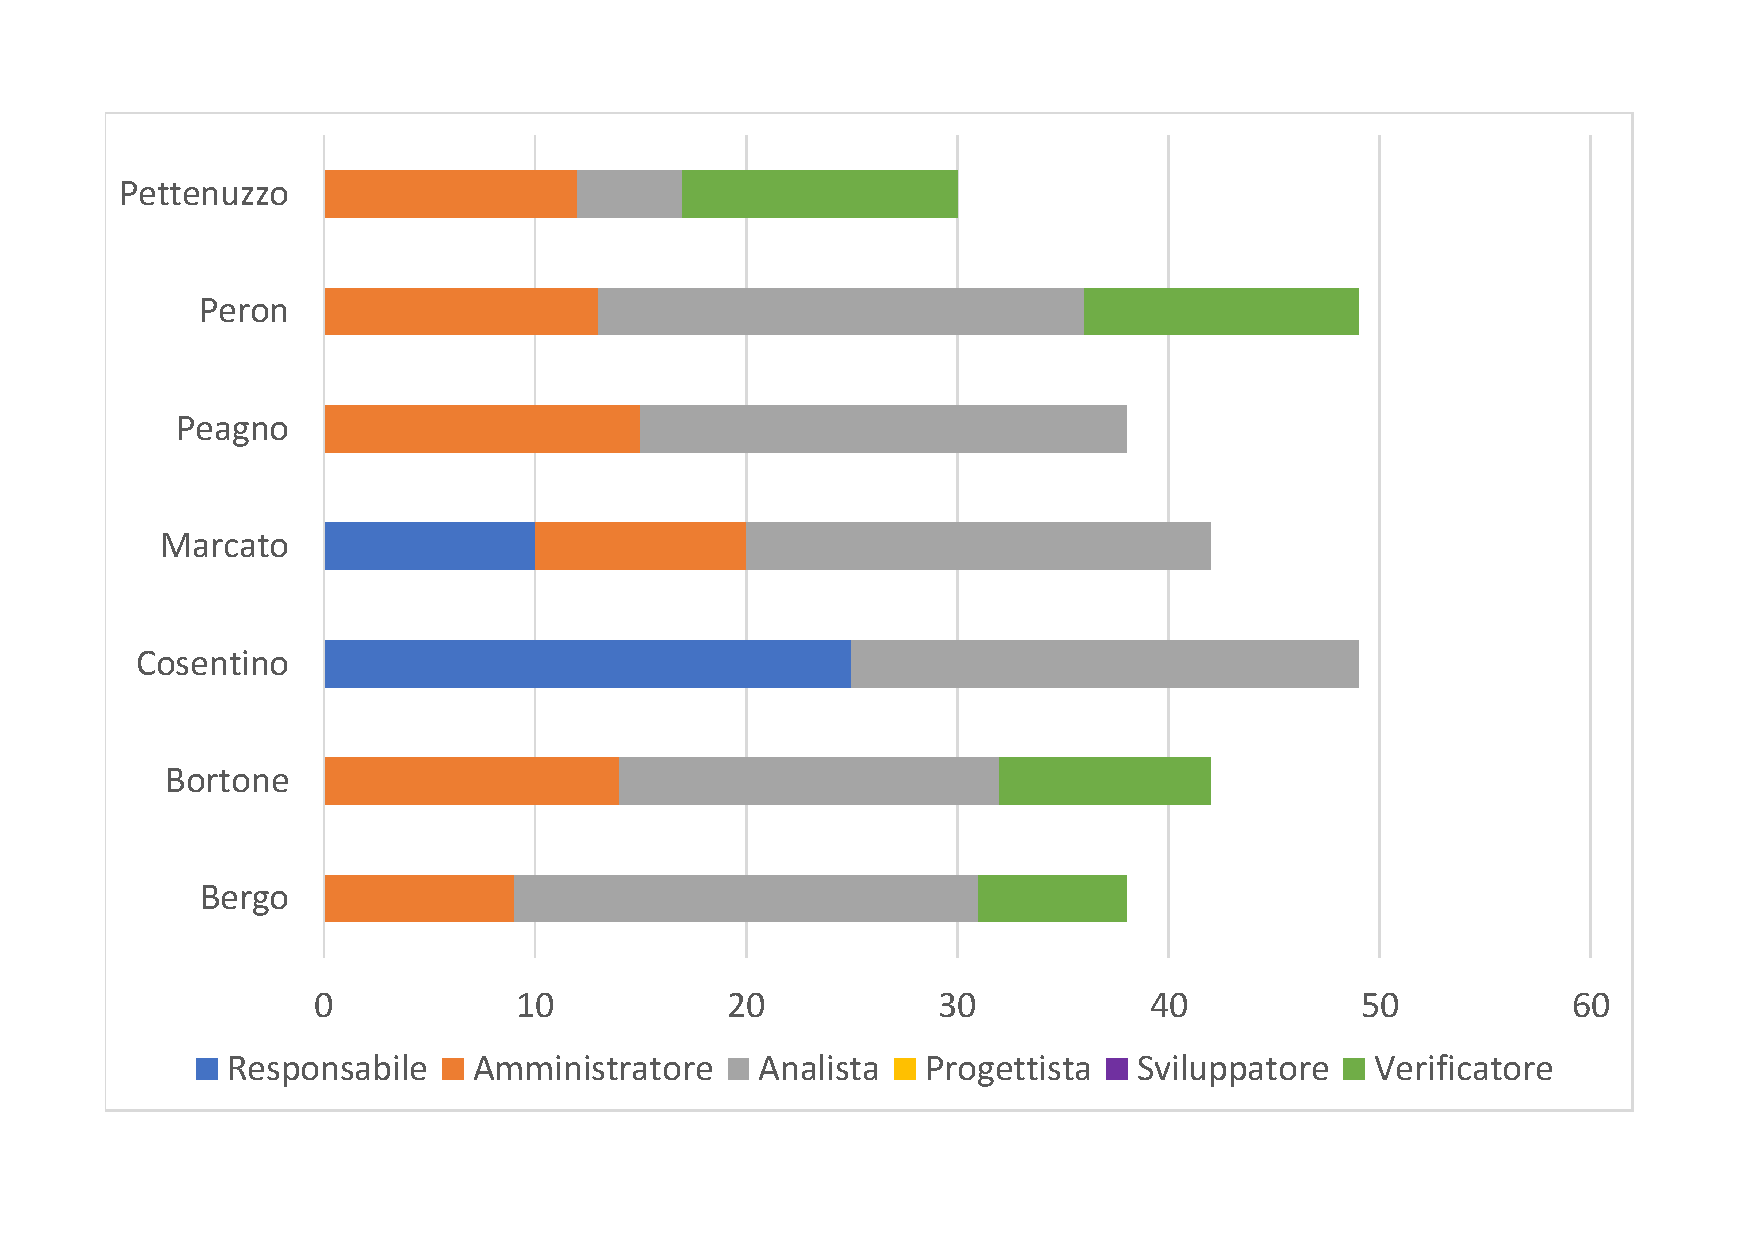
\includegraphics[scale=0.45]{images/consuntivoRR.pdf}
		\caption{Istogramma del consuntivo della fase 1}
	\end{figure}
	
	\subsubsection{Costo}
	Le seguenti tabelle indicano i costi della fase 1. Nell'ultima colonna vengono indicate le differenze tra costi previsti e costi effettivi ($previsto - effettivo$): valori positivi indicano i risparmi e valori negativi indicano le perdite.
	
	\begin{table}[H]
		\centering
		\begin{tabular}{| l | l | l |}
			\rowcolor{LightBlue}
			\textbf{\color{white}Membro}
			& \textbf{\color{white}Costo}
			& \textbf{\color{white}Differenza}\\			
			Bergo 				& 835€ 	& -65€\\
			Bortone 			& 880€ 	& -185€\\
			Cosentino 		& 1350€ 	& -125€\\
			Marcato 			& 1050€ 	& -30€\\
			Peagno 			& 875€ 	& +170€\\
			Peron 				& 1030€ 	& -30€\\
			Pettenuzzo 	& 560€ 	& +290€\\ \hline
			\textbf{Totale} & 6580€ & +25€\\ \hline
		\end{tabular}
		\caption{Costo effettivo di ciascun membro nella fase 1}	
	\end{table}

	\begin{table}[H]
		\centering
		\begin{tabular}{| l | l |l|}
			\rowcolor{LightBlue}
			\textbf{\color{white}Membro}
			& \textbf{\color{white}Costo}
			& \textbf{\color{white}Differenza}\\
			Responsabile 		& 1050€ 	& -150€\\
			Amministratore 	& 1460€ 	& +40€\\
			Analista 				& 3425€ 	& +225€\\
			Progettista 			& 0€ 		& 0€\\
			Programmatore 		& 0€ 		& 0€\\
			Verificatore 		& 645€ 	& -90€\\ \hline
			\textbf{Totale} 	& 6580€ 	& +25€\\ \hline
		\end{tabular}
		\caption{Costo effettivo di ciascun ruolo nella fase 1}
	\end{table}

	\subsubsection{Conclusioni}
		\paragraph{Costi\\}
La cifra prevista per l'investimento era di \textbf{6605€} e vi è stato un risparmio di \textbf{25€}. I costi effettivi ammontano, quindi, a \textbf{6580€}. 
		\paragraph{Scostamenti\\}
Vi sono stati dei leggeri scostamenti rispetto a quanto previsto. Ciò è imputabile a una previsione troppo pessimista delle ore necessarie per ogni attività. Tuttavia, un altro motivo può essere individuato nel mancato rispetto delle assegnazioni delle attività. Ciò è stato causato dalla frenesia da cui si è fatto prendere il gruppo nella parte successiva al periodo natalizio. Infatti, tra il 2018-12-21 e il 2019-01-06 i tempi non sono stati rispettati a causa di problemi di comunicazione tra i membri del gruppo. In seguito, a queste considerazioni è stato aggiunto alla tabella in §2.1 il rischio G03.

\newpage	
\subsection{Fase 2 (2019-01-22 - 2019-03-15)}
	\subsubsection{Ore impiegate}
La seguente tabella indica le ore impiegate durante la fase 2. Tra parentesi viene indicata la differenza tra ore preventivate e ore impiegate ($preventivo - consuntivo$): valori positivi indicano le ore risparmiate e valori negativi indicano le ore in eccesso.

		\begin{table}[H]
			\centering
		\begin{tabular}{| l | c c c c c c | c |}
			\rowcolor{LightBlue}
			& \multicolumn{7}{c}{\textbf{\color{white}Numero di ore}}	\\
	
			\rowcolor{LightBlue}
			\textbf{\color{white}Membro}
			& \textbf{\color{white}RES}
			& \textbf{\color{white}AMM}
			& \textbf{\color{white}AN}
			& \textbf{\color{white}PRO}
			& \textbf{\color{white}DEV}
			& \textbf{\color{white}VER}
			& \textbf{\color{white}Totali}\\
			Bergo     		& -  (0)		& 5  (0) 	& -  (0) 		& 18 (-3) & 10 (0) & 5  (0) 	& 38\\
			Bortone   		& -  (0)		& -  (0) 	& -  (0) 		& 22 (-1) & 9 (0) & -  (0)	& 31\\
			Cosentino 		& -  (0)	 	& -  (0) 	& 7  (-2) 		& 15 (-2) & 5 (0) & 5  (0)	& 32\\
			Marcato   		& -  (0) 		& 10  (0) 	& -  (0) 		& 10 (0) & 7 (0) & 5  (0)	& 32\\
			Peagno    		& -  (0) 		& 8  (0) 	& -  (0) 		& 10 (6) & - (0) & 10  (0)	& 28\\
			Peron     		& 15  (0)		& -  (0) 	& -  (0) 		& 13 (-3) & 10 (0) & -  (0)	& 38\\
			Pettenuzzo 		& 15  (0) 		& -  (0) 	& 8  (2) 		& 7 (-2) & - (0) & -  (0)	& 30\\ \hline
		\end{tabular}
		\caption{Ore di lavoro impiegate per membro/ruolo della fase 2}
	\end{table}
	
	\begin{figure}[H]
		\centering
		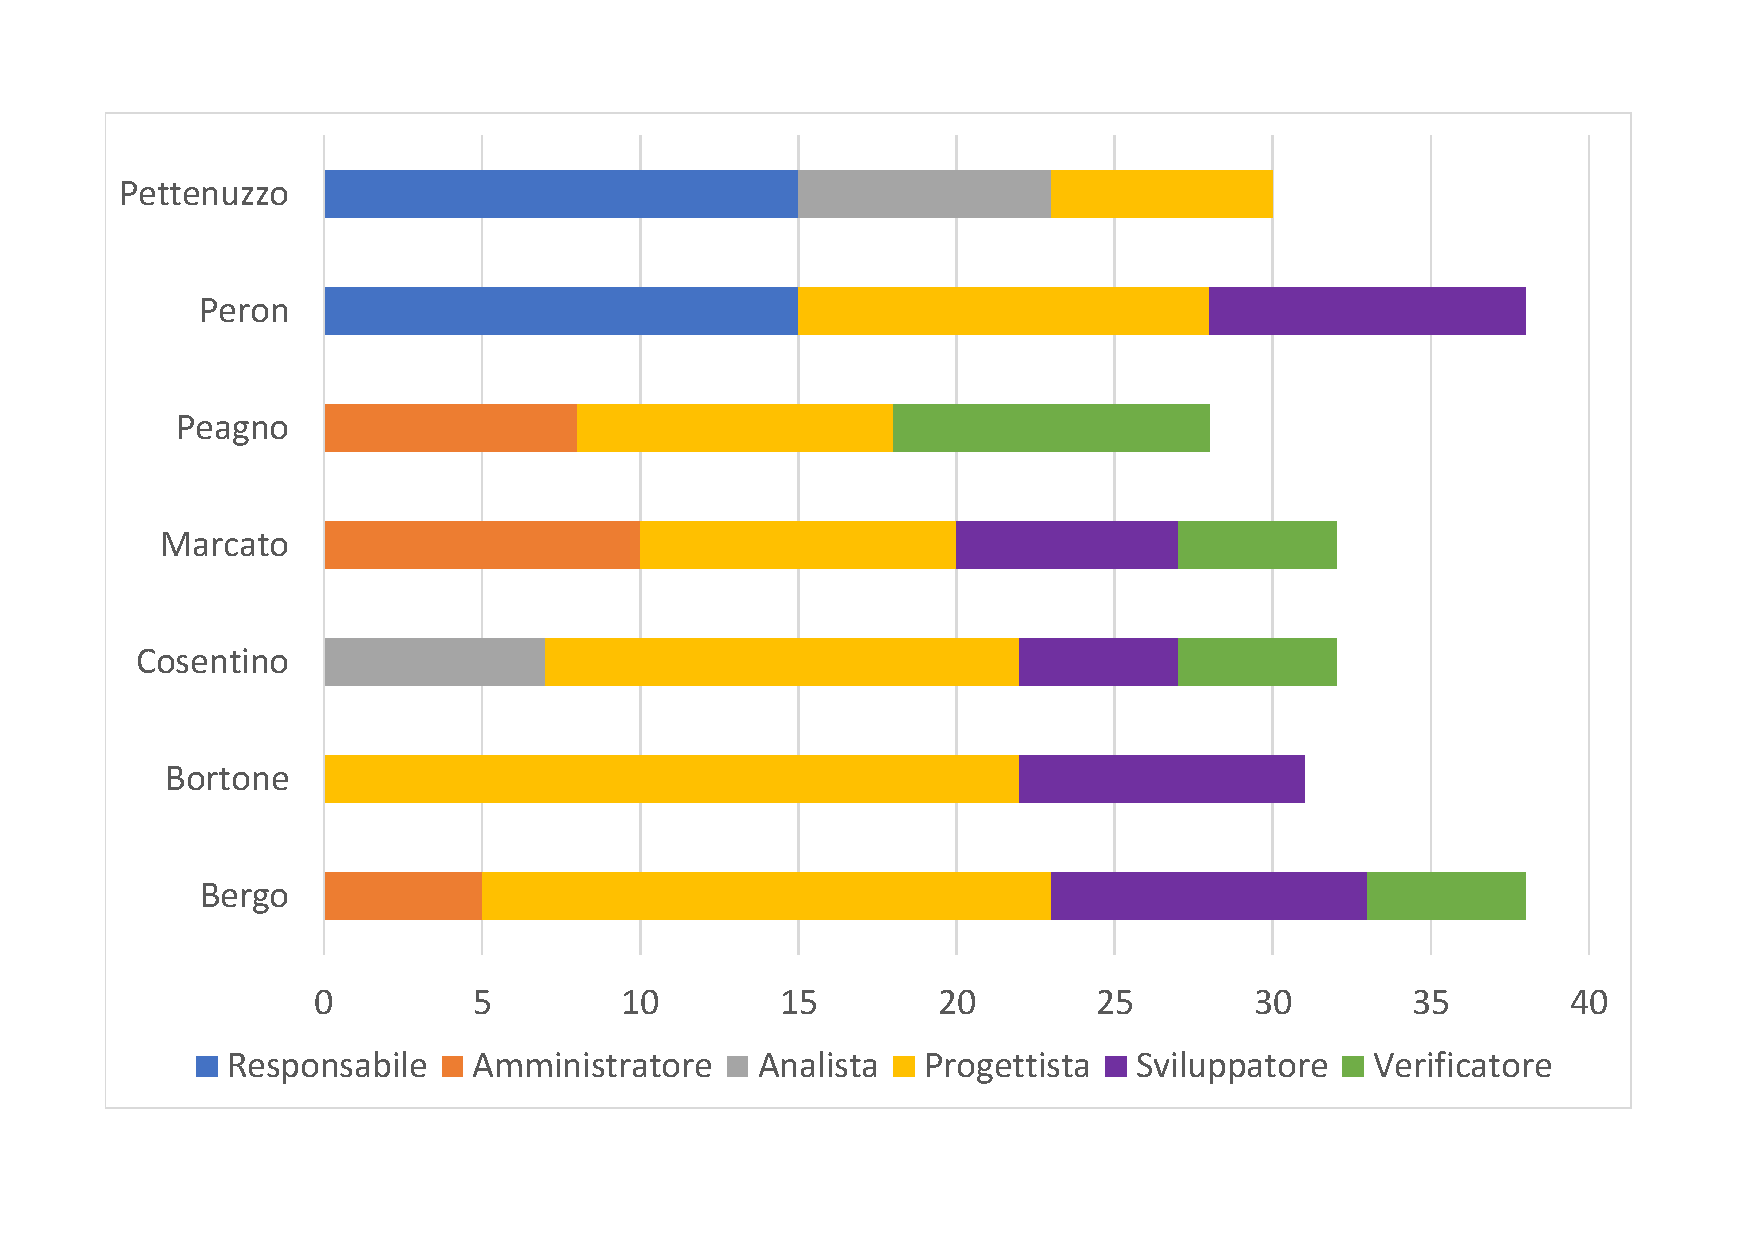
\includegraphics[scale=0.45]{images/consuntivoRP.pdf}
		\caption{Istogramma del consuntivo della fase 2}
	\end{figure}
	
	\subsubsection{Costo}
	Le seguenti tabelle indicano i costi della fase 2. Nell'ultima colonna vengono indicate le differenze tra costi previsti e costi effettivi ($previsto - effettivo$): valori positivi indicano i risparmi e valori negativi indicano le perdite.
		
	\begin{table}[H]
		\centering
		\begin{tabular}{| l | l | l |}
			\rowcolor{LightBlue}
			\textbf{\color{white}Membro}
			& \textbf{\color{white}Costo}
			& \textbf{\color{white}Differenza}\\
			Bergo		& 721€	& 9€\\
			Bortone		& 619€	& 53€\\
			Cosentino	& 655€	& -94€\\
			Marcato		& 600€	& 0€\\
			Peagno		& 530€	& 52€\\
			Peron		& 886€	& -66€\\
			Pettenuzzo	& 804€	& 6€\\ \hline
			\textbf{Totale} & 4815	& -40€\\ \hline
		\end{tabular}
		\caption{Costo effettivo di ciascun membro nella fase 2}	
	\end{table}
	
	\begin{table}[H]
		\centering
		\begin{tabular}{| l | l |l|}
			\rowcolor{LightBlue}
			\textbf{\color{white}Membro}
			& \textbf{\color{white}Costo}
			& \textbf{\color{white}Differenza}\\

			Responsabile	& 900€	& 0€\\
			Amministratore 	& 460€ 	& -80€\\
			Analista 		& 375€ 	& 0€\\
			Progettista 	& 2090€	& -110€\\
			Programmatore 	& 615€	& 150€\\
			Verificatore 	& 375€	& 0€\\ \hline
			\textbf{Totale} & 4815€	& -40€\\ \hline
		\end{tabular}
		\caption{Costo effettivo di ciascun ruolo nella fase 2}
	\end{table}
	
	\subsubsection{Conclusioni}
		\paragraph{Costi\\}
La cifra prevista per l'investimento era di \textbf{4775€}, il costo effettivo si è rivelato con un aumento di \textbf{40€} rispetto alla stima iniziale. Per cui la cifra alla fine della fase 2 corrisponde a \textbf{4815€}.
 		
		\paragraph{Scostamenti\\}
Il gruppo ha riscontrato delle difficoltà nella progettazione del Proof of Concept, la quale ha richiesto più ore rispetto a quanto preventivato. Le difficoltà derivano da una scelta tecnologica che si è rivelata errata per questo motivo sono state prese come alternativa tecnologie già conosciute dai componenti. In questo modo le ore di codifica sono state rispettate in modo soddisfacente senza grandi imprevisti.
\newpage
\subsection{Fase 3 (2019-03-16 - 2019-04-19)}
	\subsubsection{Ore impiegate}
	La seguente tabella indica le ore impiegate durante la fase 3. Tra parentesi viene indicata la differenza tra ore preventivate e ore impiegate ($preventivo - consuntivo$): valori positivi indicano le ore risparmiate e valori negativi indicano le ore in eccesso.
	
	\begin{table}[H]
		\centering
		\begin{tabular}{| l | c c c c c c | c |}
			\rowcolor{LightBlue}
			& \multicolumn{7}{c}{\textbf{\color{white}Numero di ore}}	\\
			
			\rowcolor{LightBlue}
			\textbf{\color{white}Membro}
			& \textbf{\color{white}RES}
			& \textbf{\color{white}AMM}
			& \textbf{\color{white}AN}
			& \textbf{\color{white}PRO}
			& \textbf{\color{white}DEV}
			& \textbf{\color{white}VER}
			& \textbf{\color{white}Totali}\\
			Bergo     		& 15  (0) & 2 (+2) 	& -  (0) 		& 8 (-2) & 10 (0) & 10 (0) 	& 45\\
			Bortone   		& 11  (-4) & -  (0) 	& -  (-5) 		& 8 (0) & 16 (+9) & 12 (+2)	& 47\\
			Cosentino & - (0) & 5 (0) 	& 2 (+2) & 21 (0) & 18 (-3) & - (0)	& 46\\
			Marcato  & -  (0) & 5 (+5) 	& -  (0) & 15 (-10) & 26 (+1) & - (0) & 46\\
			Peagno    		& -  (0) & - (0) & -  (0) & 20 (-5) & 27 (+2) & - (0)	& 47\\
			Peron   & -  (0) & -  (0) 	& -  (0) & 15 (0) & 20 (+5) &  10 (-5)	& 45\\
			Pettenuzzo 		& - (0) & 5 (+5) & 3 (-2) & 8 (-2) & 26 (+1) & 10 (0)	& 52\\ \hline
		\end{tabular}
		\caption{Ore di lavoro impiegate per membro/ruolo della fase 3}
		
		\begin{figure}[H]
			\centering
			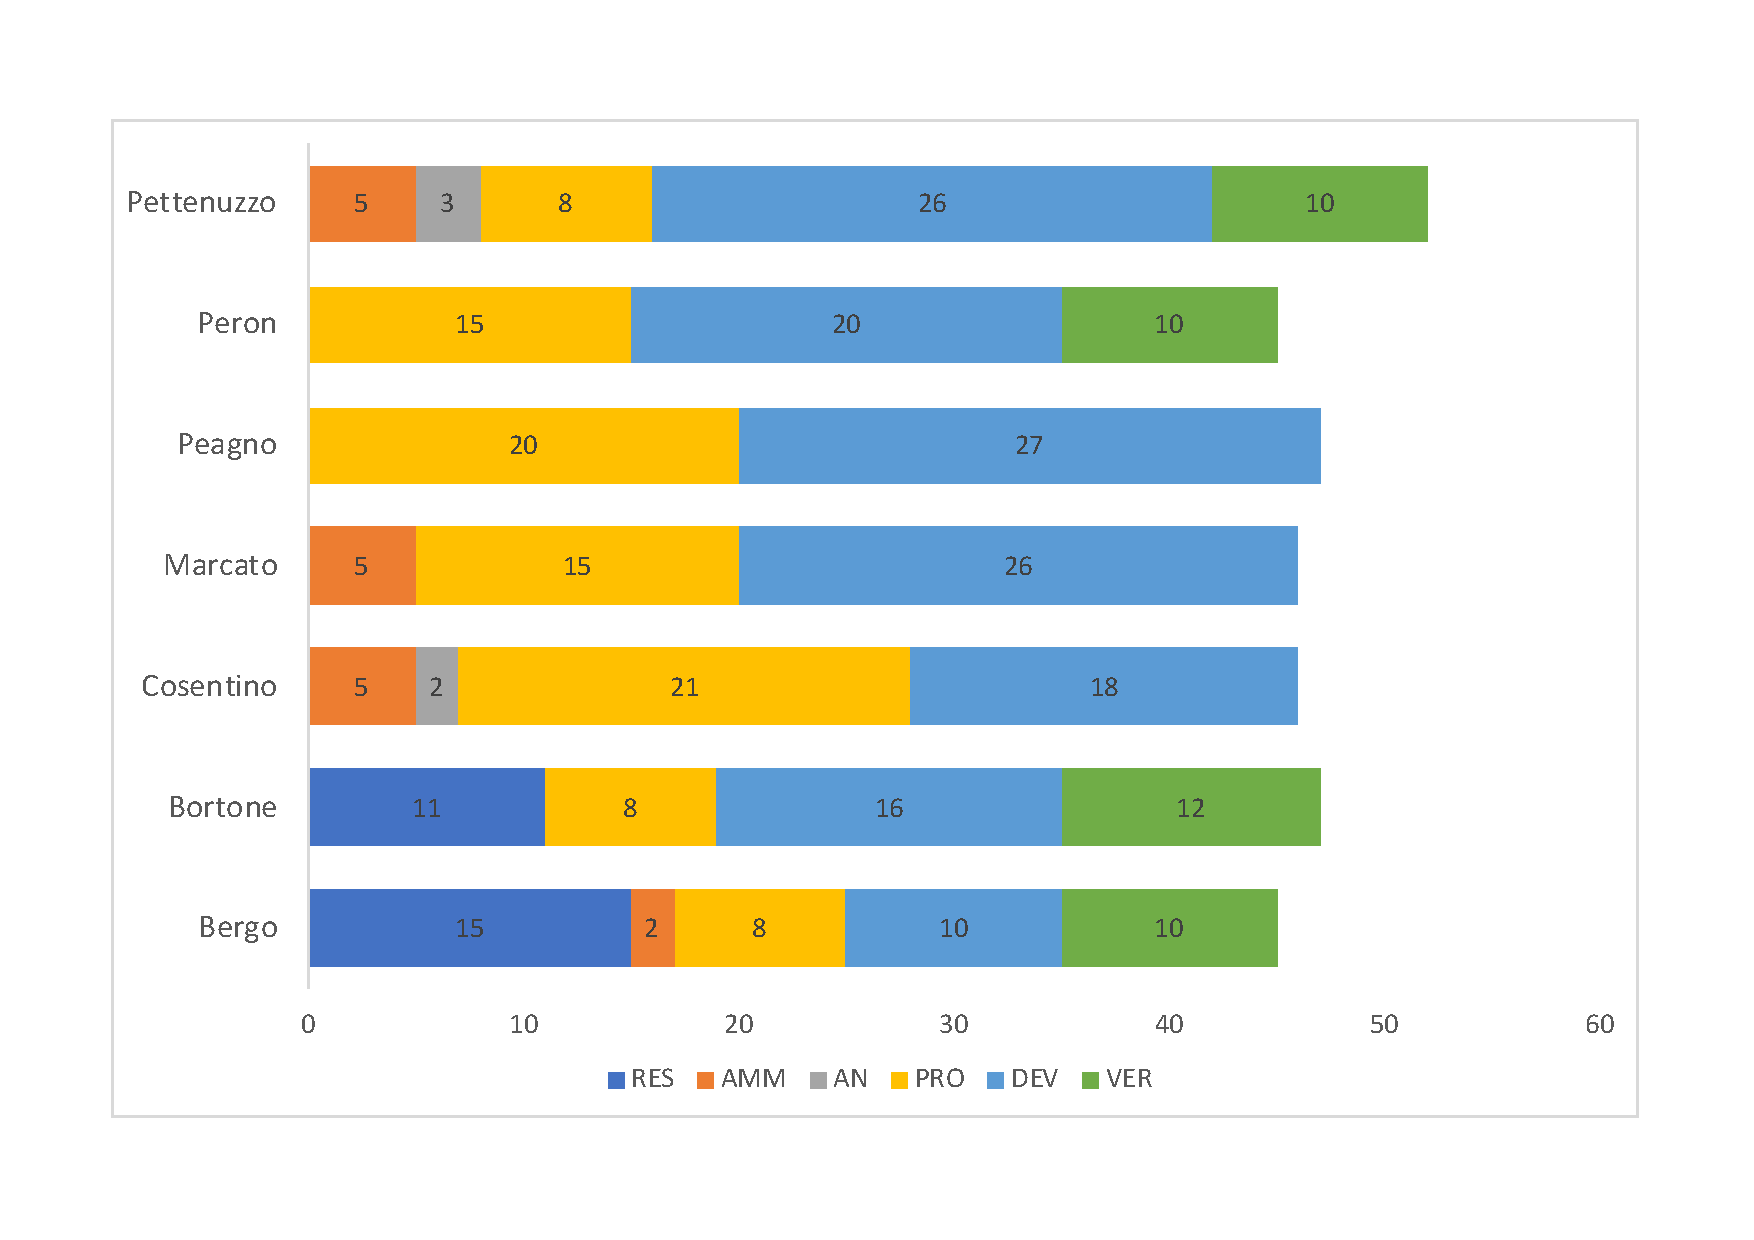
\includegraphics[scale=0.45]{images/consuntivoRQ.pdf}
			\caption{Istogramma del consuntivo della fase 3}
		\end{figure}
		
		
	\end{table}
	\subsubsection{Costo}
		Le seguenti tabelle indicano i costi della fase 3. Nell'ultima colonna vengono indicate le differenze tra costi previsti e costi effettivi ($previsto - effettivo$): valori positivi indicano i risparmi e valori negativi indicano le perdite.
		
		\begin{table}[H]
			\centering
			\begin{tabular}{| l | l | l |}
				\rowcolor{LightBlue}
				\textbf{\color{white}Membro}
				& \textbf{\color{white}Costo}
				& \textbf{\color{white}Differenza}\\
				Bergo		& 966€	& 4€\\
				Bortone		& 926€	& 80€\\
				Cosentino	& 882€	& -5€\\
				Marcato		& 820€	& 105€\\
				Peagno		& 845€	& 80€\\
				Peron		& 780€	& 0€\\
				Pettenuzzo	& 891€	& -21€\\ \hline
				\textbf{Totale} & 6110	& 243€\\ \hline
			\end{tabular}
			\caption{Costo effettivo di ciascun membro nella fase 3}	
		\end{table}
	
	
	\begin{table}[H]
		\centering
		\begin{tabular}{| l | l |l|}
			\rowcolor{LightBlue}
			\textbf{\color{white}Membro}
			& \textbf{\color{white}Costo}
			& \textbf{\color{white}Differenza}\\
			
			Responsabile	& 780€	& 120€\\
			Amministratore 	& 340€ 	& -240€\\
			Analista 		& 125€ 	& 125€\\
			Progettista 	& 2090€	& 418€\\
			Programmatore 	& 2145€	& -225€\\
			Verificatore 	& 630€	& 45€\\ \hline
			\textbf{Totale} & 6110€	& 243€\\ \hline
		\end{tabular}
		\caption{Costo effettivo di ciascun ruolo nella fase 3}
	\end{table}


	\subsubsection{Gestione dei rischi}
	Durante lo svolgersi di questa fase, nessuno dei rischi elencati in \S2 si è verificato. Abbiamo provveduto ad abbassare la probabilità o pericolo dei seguenti rischi: 
	\begin{itemize}
	\item 		O01 Superamento dei costi: dato che il progetto è in una fase avanzata, è più semplice pianificare e conseguentemente più facile rientrare nei costi;
	\item 		G03 Problemi di comunicazione: il team è riuscito a comunicare in maniera più tempestiva;
	\item		T01 Tecnologie da applicare: le tecnologie applicate in questa fase sono già ben comprese dal team;
	\item 		G02 Contrasti nel team: ormai il team si conosce, mostrando certe affinità caratteriali ed il rischio è quasi nullo.
	\end{itemize}

	La pianificazione della fase 4 è stata modificata in base a questo consuntivo.
	\subsubsection{Conclusioni}
	\paragraph{Costi\\}\noindent\\
 La cifra prevista per l'investimento era di \textbf{6353€}, il costo effettivo è diminuito rispetto alla stima iniziale. Per cui la cifra alla fine della fase 3 è di \textbf{6110€}.Tenendo conto dell'aumento di \textbf{40€} della fase precedente il costo effettivo è \textbf{6150€}.
I rimasti \textbf{203€} saranno reinvestiti nella successiva fase.

\paragraph{Scostamenti\\}\noindent\\

	\newpage
	\subsection{Preventivo a finire}
La seguente tabella presenta l'attuale preventivo a finire. Se il valore del consuntivo di un determinato periodo non è ancora presente, per il conteggio totale verrà utilizzato il valore del preventivo.

\begin{table}[H]
			\centering
		\begin{tabular}{| l | l | l | l |}
			\rowcolor{LightBlue}
			\textbf{\color{white}Fase}
			& \textbf{\color{white}Preventivo}
			& \textbf{\color{white}Consuntivo}
			& \textbf{\color{white}Variazione}
			\\
			
			Fase 2 			& 4775€ 	& 4815€ & -40€\\
			Fase 3 		& 6353€ 	& - & -\\
			Fase 4			& 3037€ 	& - & -\\
			\textbf{Totale} & 14090€ & 14105€ & -15€\\ \hline
		\end{tabular}
		\caption{Preventivo a finire aggiornato al termine della fase 2}	
\end{table}
La cifra risparmiata durante la fase 1 non è stata reinvestita durante la modifica della pianificazione. La variazione ($preventivo - consuntivo$) quindi è di -15, è necessario un maggiore impegno da parte del gruppo nelle fasi successive per rientrare nel costo preventivato in partenza. 

\newpage

	\appendix
	\section{Organigramma}
%		\input{appendiceA.tex}
\end{document}